\documentclass[11pt,a4paper]{article}
\usepackage{fontspec}
\setmainfont{Latin Modern Roman}
\setsansfont{Latin Modern Sans}
\setmonofont{Latin Modern Mono}
\usepackage{microtype}
\usepackage[margin=2.2cm,headheight=14pt]{geometry}
\usepackage{graphicx}
\usepackage{booktabs,longtable,tabularx,array,multirow}
\usepackage[table]{xcolor}
\usepackage{listings}
\usepackage[most]{tcolorbox}
\usepackage{enumitem}
\usepackage{fancyhdr}
\usepackage{caption}
\usepackage{float}
\usepackage{amssymb}
\usepackage[hidelinks]{hyperref}
\usepackage{bookmark}

\newcommand{\ramA}{8.2}
\newcommand{\ramB}{6.0}


\definecolor{tviblue}{HTML}{1F3864}
\definecolor{codebg}{HTML}{F6F8FA}
\definecolor{planeA}{HTML}{1F77B4}
\definecolor{planeB}{HTML}{D9711C}

\lstdefinestyle{cfg}{basicstyle=\ttfamily\scriptsize,backgroundcolor=\color{codebg},frame=single,
  rulecolor=\color{black!20},breaklines=true,columns=fullflexible,keepspaces=true,
  showstringspaces=false,xleftmargin=2pt,xrightmargin=2pt,aboveskip=6pt,belowskip=6pt}
\lstset{style=cfg}

\newcounter{evid}
\newcommand{\evidence}[2]{%
  \refstepcounter{evid}%
  \begin{tcolorbox}[enhanced,breakable,colback=yellow!7,colframe=orange!75!black,boxrule=0.5pt,
     title={Evidence E\theevid\ -- #1},fonttitle=\small\bfseries,left=4pt,right=4pt,top=2pt,bottom=2pt]
  \small Command(s): \texttt{#2}\\[2pt]
  \itshape [Paste the real CLI output or a cropped screenshot captured in the EVE-NG lab here, then delete this line.]
  \end{tcolorbox}}

\makeatletter\newcommand{\tabin}[1]{\@@input #1 }\makeatother
\newcommand{\todo}[1]{\colorbox{yellow!40}{\textbf{TODO:} #1}}

\pagestyle{fancy}
\fancyhf{}
\lhead{\small TVI Enterprise Network -- Technical Explanation Report}
\rhead{\small Computer Networks -- Assignment 2}
\cfoot{\small \thepage}
\renewcommand{\headrulewidth}{0.4pt}

\setlength{\parskip}{4pt}
\setlength{\parindent}{0pt}
\setlist{itemsep=2pt,topsep=3pt}
\renewcommand{\arraystretch}{1.15}

\begin{document}

% ======================================================================== cover
\begin{titlepage}
\centering
{\large VIETNAM NATIONAL UNIVERSITY HO CHI MINH CITY\\
HO CHI MINH CITY UNIVERSITY OF TECHNOLOGY\\
FACULTY OF COMPUTER SCIENCE AND ENGINEERING\par}
\vspace{2.5cm}
{\Large COMPUTER NETWORKING \& NETWORK ADMINISTRATION\par}
\vspace{0.6cm}
{\Large Assignment 2\par}
\vspace{1.0cm}
{\color{tviblue}\rule{\linewidth}{1pt}\\[0.4cm]
{\huge\bfseries Large Enterprise Network Design\\[0.2cm] and Implementation\par}
\vspace{0.3cm}
{\Large TechViet Innovations (TVI) -- Technical Explanation Report\par}
\rule{\linewidth}{1pt}}
\vspace{1.6cm}

\begin{tabular}{lll}
\toprule
\textbf{No.} & \textbf{Full name} & \textbf{Student ID}\\
\midrule
1 & Phạm Minh Đức & 2414106\\
2 & \todo{member 2} & \\
3 & \todo{member 3} & \\
4 & \todo{member 4} & \\
\bottomrule
\end{tabular}

\vspace{1cm}
Lab group: \todo{group} \qquad Instructor: \todo{instructor}

\vfill
{\large Ho Chi Minh City, November 2026\par}
\end{titlepage}

\tableofcontents
\listoffigures
\listoftables
\clearpage

% ======================================================================== 1
\section{Executive Summary}

TechViet Innovations (TVI) operates three sites -- the Ho Chi Minh City headquarters and data centre (2,000+ users), the Hanoi R\&D campus (1,500+ users with AI training workloads) and the Da Nang logistics hub (500+ users and the bulk of more than 10,000 IoT endpoints) -- over a flat hub-and-spoke WAN. The current design forces every branch flow, including traffic to cloud applications, through headquarters, relies on large broadcast domains that are prone to broadcast storms, and protects the company only at a single perimeter. These weaknesses translate directly into slow SaaS access in Hanoi and Da Nang, outages whenever the single HQ path fails, and a flat internal network in which a compromised IoT scanner can reach the finance department.

This report presents a replacement architecture and a working virtual implementation of it. The design rests on four decisions, each tied to a business problem:

\begin{enumerate}
\item \textbf{No single point of failure.} Every site has two WAN edge routers on two independent carriers, every campus gateway is a redundant HSRP pair, and HQ core links are bundled with LACP. Loss of any one link, router or carrier is absorbed in seconds, which is the precondition for the 99.99\,\% (about 53 minutes per year) availability target.
\item \textbf{Direct, secure site-to-site and cloud access.} Sites are connected by an SD-WAN-style overlay: a full mesh of IPsec-encrypted tunnels on each carrier, with BGP selecting the path. Each site sends Internet and SaaS traffic directly to its local carrier, eliminating the HQ backhaul that causes today's latency.
\item \textbf{Segmentation by default.} Executives, engineers, logistics staff, voice, IoT and guests live in separate VLANs and subnets; guests reach only the Internet, IoT devices reach only the IoT platform, and the executive VLAN accepts connections only from servers and administrators. A zone-based firewall guards every Internet edge, and remote staff are served through Zero Trust Network Access rather than a flat VPN.
\item \textbf{Programmable operations.} All configurations are generated from a single source-of-truth file, checked automatically before deployment, and maintained by a Python/Netmiko tool that backs up, provisions and audits every device, so that new VLANs or policies are rolled out consistently instead of by hand.
\end{enumerate}

The addressing plan reserves a summarisable /16 IPv4 block and a /48 IPv6 block per site and is sized for the 2030 targets of 10,000 users and more than 25,000 IoT endpoints without renumbering. Voice receives strict priority on every WAN link. The design was implemented in EVE-NG with Cisco vIOS/IOSvL2 (campus and WAN, \ramA\,GB of RAM) and Arista vEOS (data-centre EVPN-VXLAN fabric, \ramB\,GB), so that both labs fit the 12\,GB machines available to the team. Section~\ref{sec:testing} documents the verification and failover evidence collected from the running lab.

% ======================================================================== 2
\section{Requirement Analysis}
\label{sec:req}

\subsection{From business needs to technical requirements}

Table~\ref{tab:req} maps every need stated in the brief to the technical measure that satisfies it and to the section in which it is justified. The table also serves as the traceability matrix used to plan the test cases in Section~\ref{sec:testing}.

\begin{table}[H]
\centering\small
\caption{Business-to-technical requirement traceability}
\label{tab:req}
\begin{tabularx}{\linewidth}{@{}p{3.6cm}X p{1.2cm}@{}}
\toprule
\textbf{Business need} & \textbf{Technical measure in this design} & \textbf{Section}\\
\midrule
High availability, no SPOF at L2/L3 & Dual WAN edges and carriers per site; HSRPv2 gateway pairs; LACP Port-channel between HQ cores; Rapid-PVST+ with deterministic roots; ECMP OSPF; two independent overlay planes & \ref{sec:l2}, \ref{sec:fhrp}, \ref{sec:ha}\\
99.99\,\% uptime, 10/40\,Gbps HQ backbone & Redundant everything above; 10/40\,GbE spine-leaf fabric and core links in production; sub-5\,s gateway failover & \ref{sec:ha}\\
Broadcast storms in the flat legacy LAN & Maximum /24 per broadcast domain, VLANs pruned on trunks, root/BPDU guard, loop guard, routed (L3) uplinks above the core & \ref{sec:ip}, \ref{sec:l2}\\
Latency to SaaS from branches & Local Internet breakout with PAT at every site; overlay only for site-to-site traffic & \ref{sec:overlay}\\
Secure remote access for a hybrid workforce & ZTNA/SASE: identity-aware, per-application access brokered by a cloud PoP, no network-level VPN & \ref{sec:ztna}\\
Agility and automation (IaC) & Single source of truth renders all configs; offline validation; Python/Netmiko provisioning, backup, compliance and telemetry & \ref{sec:auto}\\
4,000 users now, 10,000 by 2030, 10k+ IoT & VLSM pools sized for 2030 per site; IPv6 /48 per site; IoT pool of 32,766 addresses at Da Nang & \ref{sec:ip}\\
Voice, video and data on one network & DSCP marking at the trust boundary, LLQ with 30\,\% strict priority for EF under a WAN shaper & \ref{sec:qos}\\
Executives: maximum security & IPsec (AES-256) on every inter-site flow; executive VLAN protected by an outbound ACL; separate VLAN and subnet & \ref{sec:sec}\\
R\&D: east-west bandwidth & Dedicated AI-lab /18 for a local spine-leaf GPU fabric; EVPN-VXLAN at HQ for the private cloud & \ref{sec:evpn}\\
Logistics: low-latency Wi-Fi 6/7 & Dense AP VLAN (/23) with controller-based roaming (CAPWAP); IoT isolated in its own VLAN & \ref{sec:wlan}\\
Guests: Internet only & Guest VLAN per site with ACL denying all RFC\,1918 space; public DNS; short leases; no IPv6 & \ref{sec:sec}\\
\bottomrule
\end{tabularx}
\end{table}

\subsection{Scope, assumptions and lab abstraction}

The \emph{design} describes the production network. The \emph{implementation} reproduces every protocol the rubric requires at a reduced scale that a 12\,GB laptop can run. Table~\ref{tab:abstraction} states each abstraction explicitly so that the reader can judge what the lab proves.

\begin{table}[H]
\centering\small
\caption{Production design versus lab implementation}
\label{tab:abstraction}
\begin{tabularx}{\linewidth}{@{}p{3.2cm}XX@{}}
\toprule
\textbf{Element} & \textbf{Production design} & \textbf{Lab A / Lab B implementation}\\
\midrule
WAN transports & Business broadband (ISP-A) and MPLS/business fibre (ISP-B) & Two vIOS routers emulating the carriers (AS 65100/65200) with an inter-carrier peering\\
SD-WAN & Commercial SD-WAN controller with application-aware routing & GRE-over-IPsec full mesh per transport, eBGP path selection, HSRP placement to split data and voice across transports\\
HQ campus & Collapsed core (2 $\times$ L3 switches) and many access stacks & 2 $\times$ IOSvL2 core, 1 IOSvL2 access switch\\
Branch campus & Two edge routers with a pair of distribution switches & Two vIOS edges as router-on-a-stick gateways (HSRP) and one access switch\\
Data centre & EVPN-VXLAN spine-leaf, border leaves to the core & Separate Lab B: 1--2 vEOS spines, 2 vEOS leaves (RAM limit)\\
Services & DHCP/DNS/NTP servers, WLC cluster, NMS & One vIOS router acting as DHCP/DNS/NTP server and VoIP probe; WLC and ZTNA are design-only\\
Endpoints & Thousands of users, phones, APs, IoT & VPCS hosts, one per VLAN\\
Addressing & 10.0.0.0/8, global IPv6 /40 & Same plan; IPv6 documentation prefix 2001:db8::/32 (RFC 3849) and IPv4 TEST-NETs (RFC 5737) for the carriers\\
\bottomrule
\end{tabularx}
\end{table}

% ======================================================================== 3
\section{Architecture and Topology}
\label{sec:arch}

\subsection{Logical architecture}

Figure~\ref{fig:logical} shows the target architecture. Each site is an autonomous routing domain with its own OSPF underlay and its own BGP autonomous system, joined to the others only through the encrypted overlay. This structure contains failures and changes within a site, keeps the routing tables of each site small (one summary per remote site), and allows a fourth site to be added by connecting two edge routers and announcing one /16.

\begin{figure}[H]
\centering
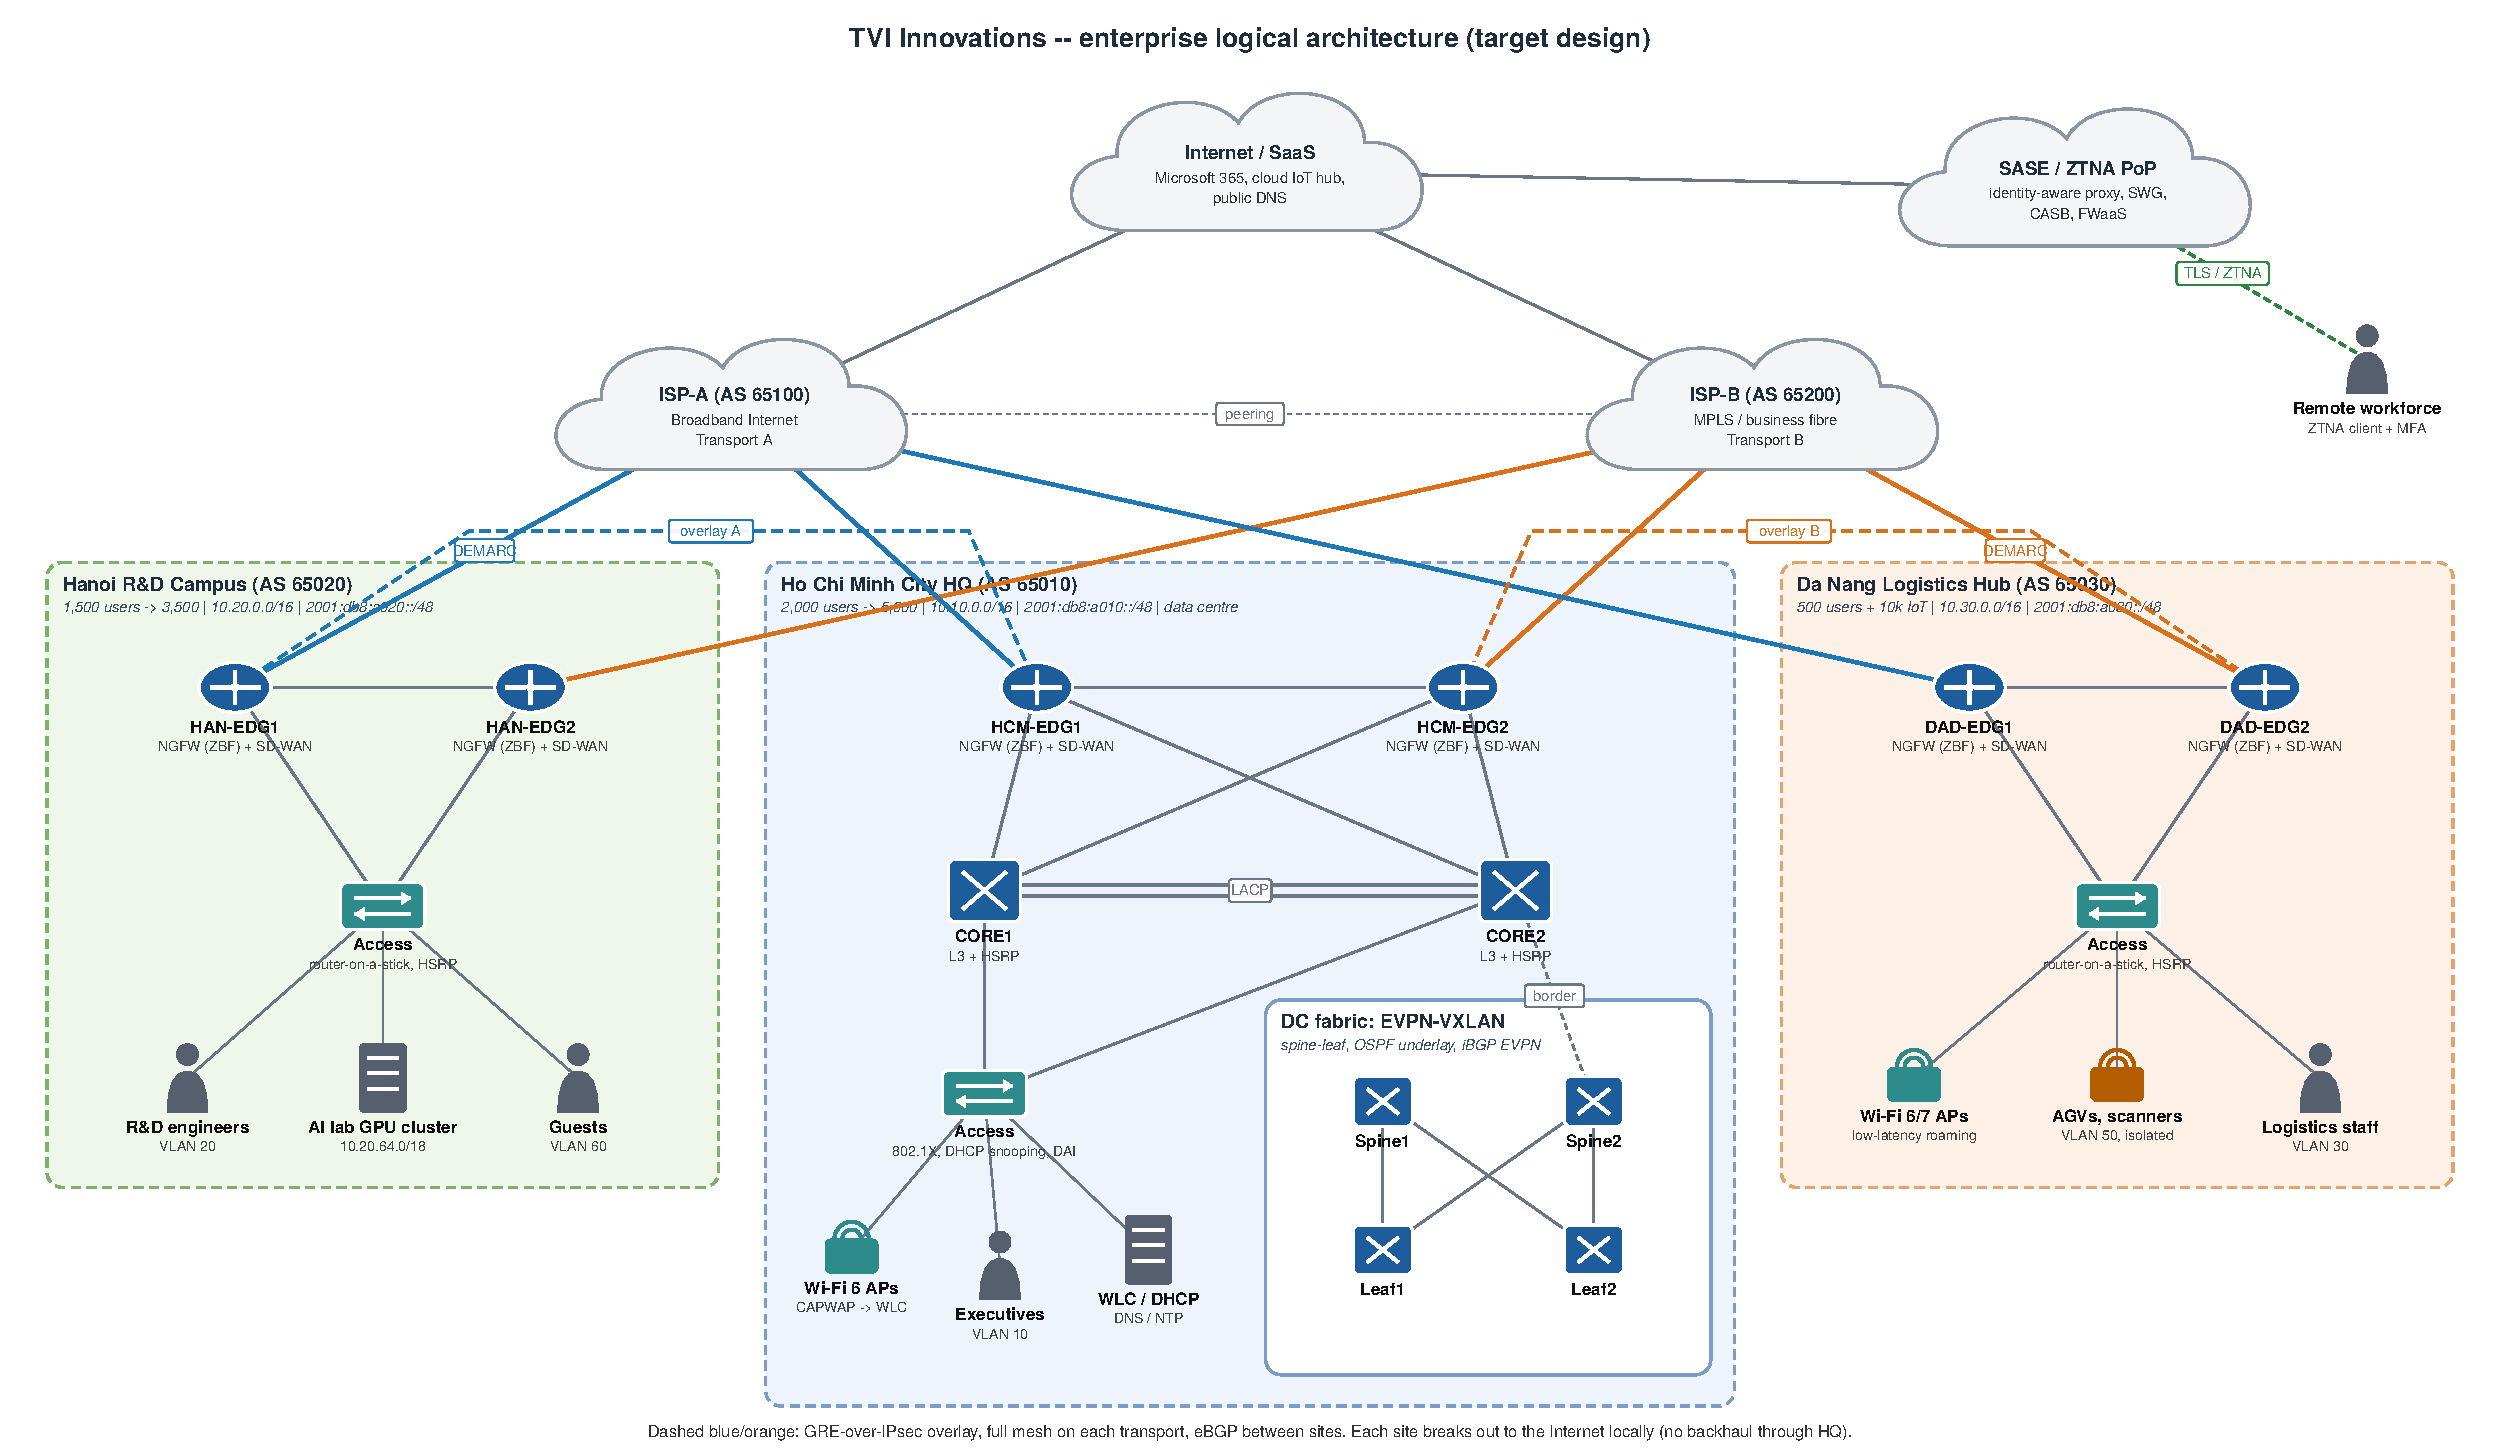
\includegraphics[width=\linewidth]{figures/01-logical-architecture.pdf}
\caption{Enterprise logical architecture with transports, overlay, campus, data centre and SASE}
\label{fig:logical}
\end{figure}

\paragraph{Demarcation points.} The boundary of TVI's responsibility is the WAN interface \texttt{Gi0/1} of each edge router (labelled \emph{DEMARC} in Figure~\ref{fig:logical} and ``demarcation point'' in the interface descriptions). Everything on the carrier side of these six /30 links belongs to ISP-A or ISP-B; TVI controls only what it sends (nothing but IPsec, IKE and BGP towards the carriers) and what it accepts (a default route only). The SASE PoP is a second, logical demarcation: remote users never touch the TVI network directly, they reach individual applications through the provider's broker.

\subsection{Physical lab topology (Lab A)}

Figure~\ref{fig:physical} is the topology built in EVE-NG, with every interface identifier and link subnet. The tables in Section~\ref{sec:ip} and the configuration files in \texttt{configs/labA/} are generated from the same data, so the labels in the figure match the devices exactly.

\begin{figure}[H]
\centering
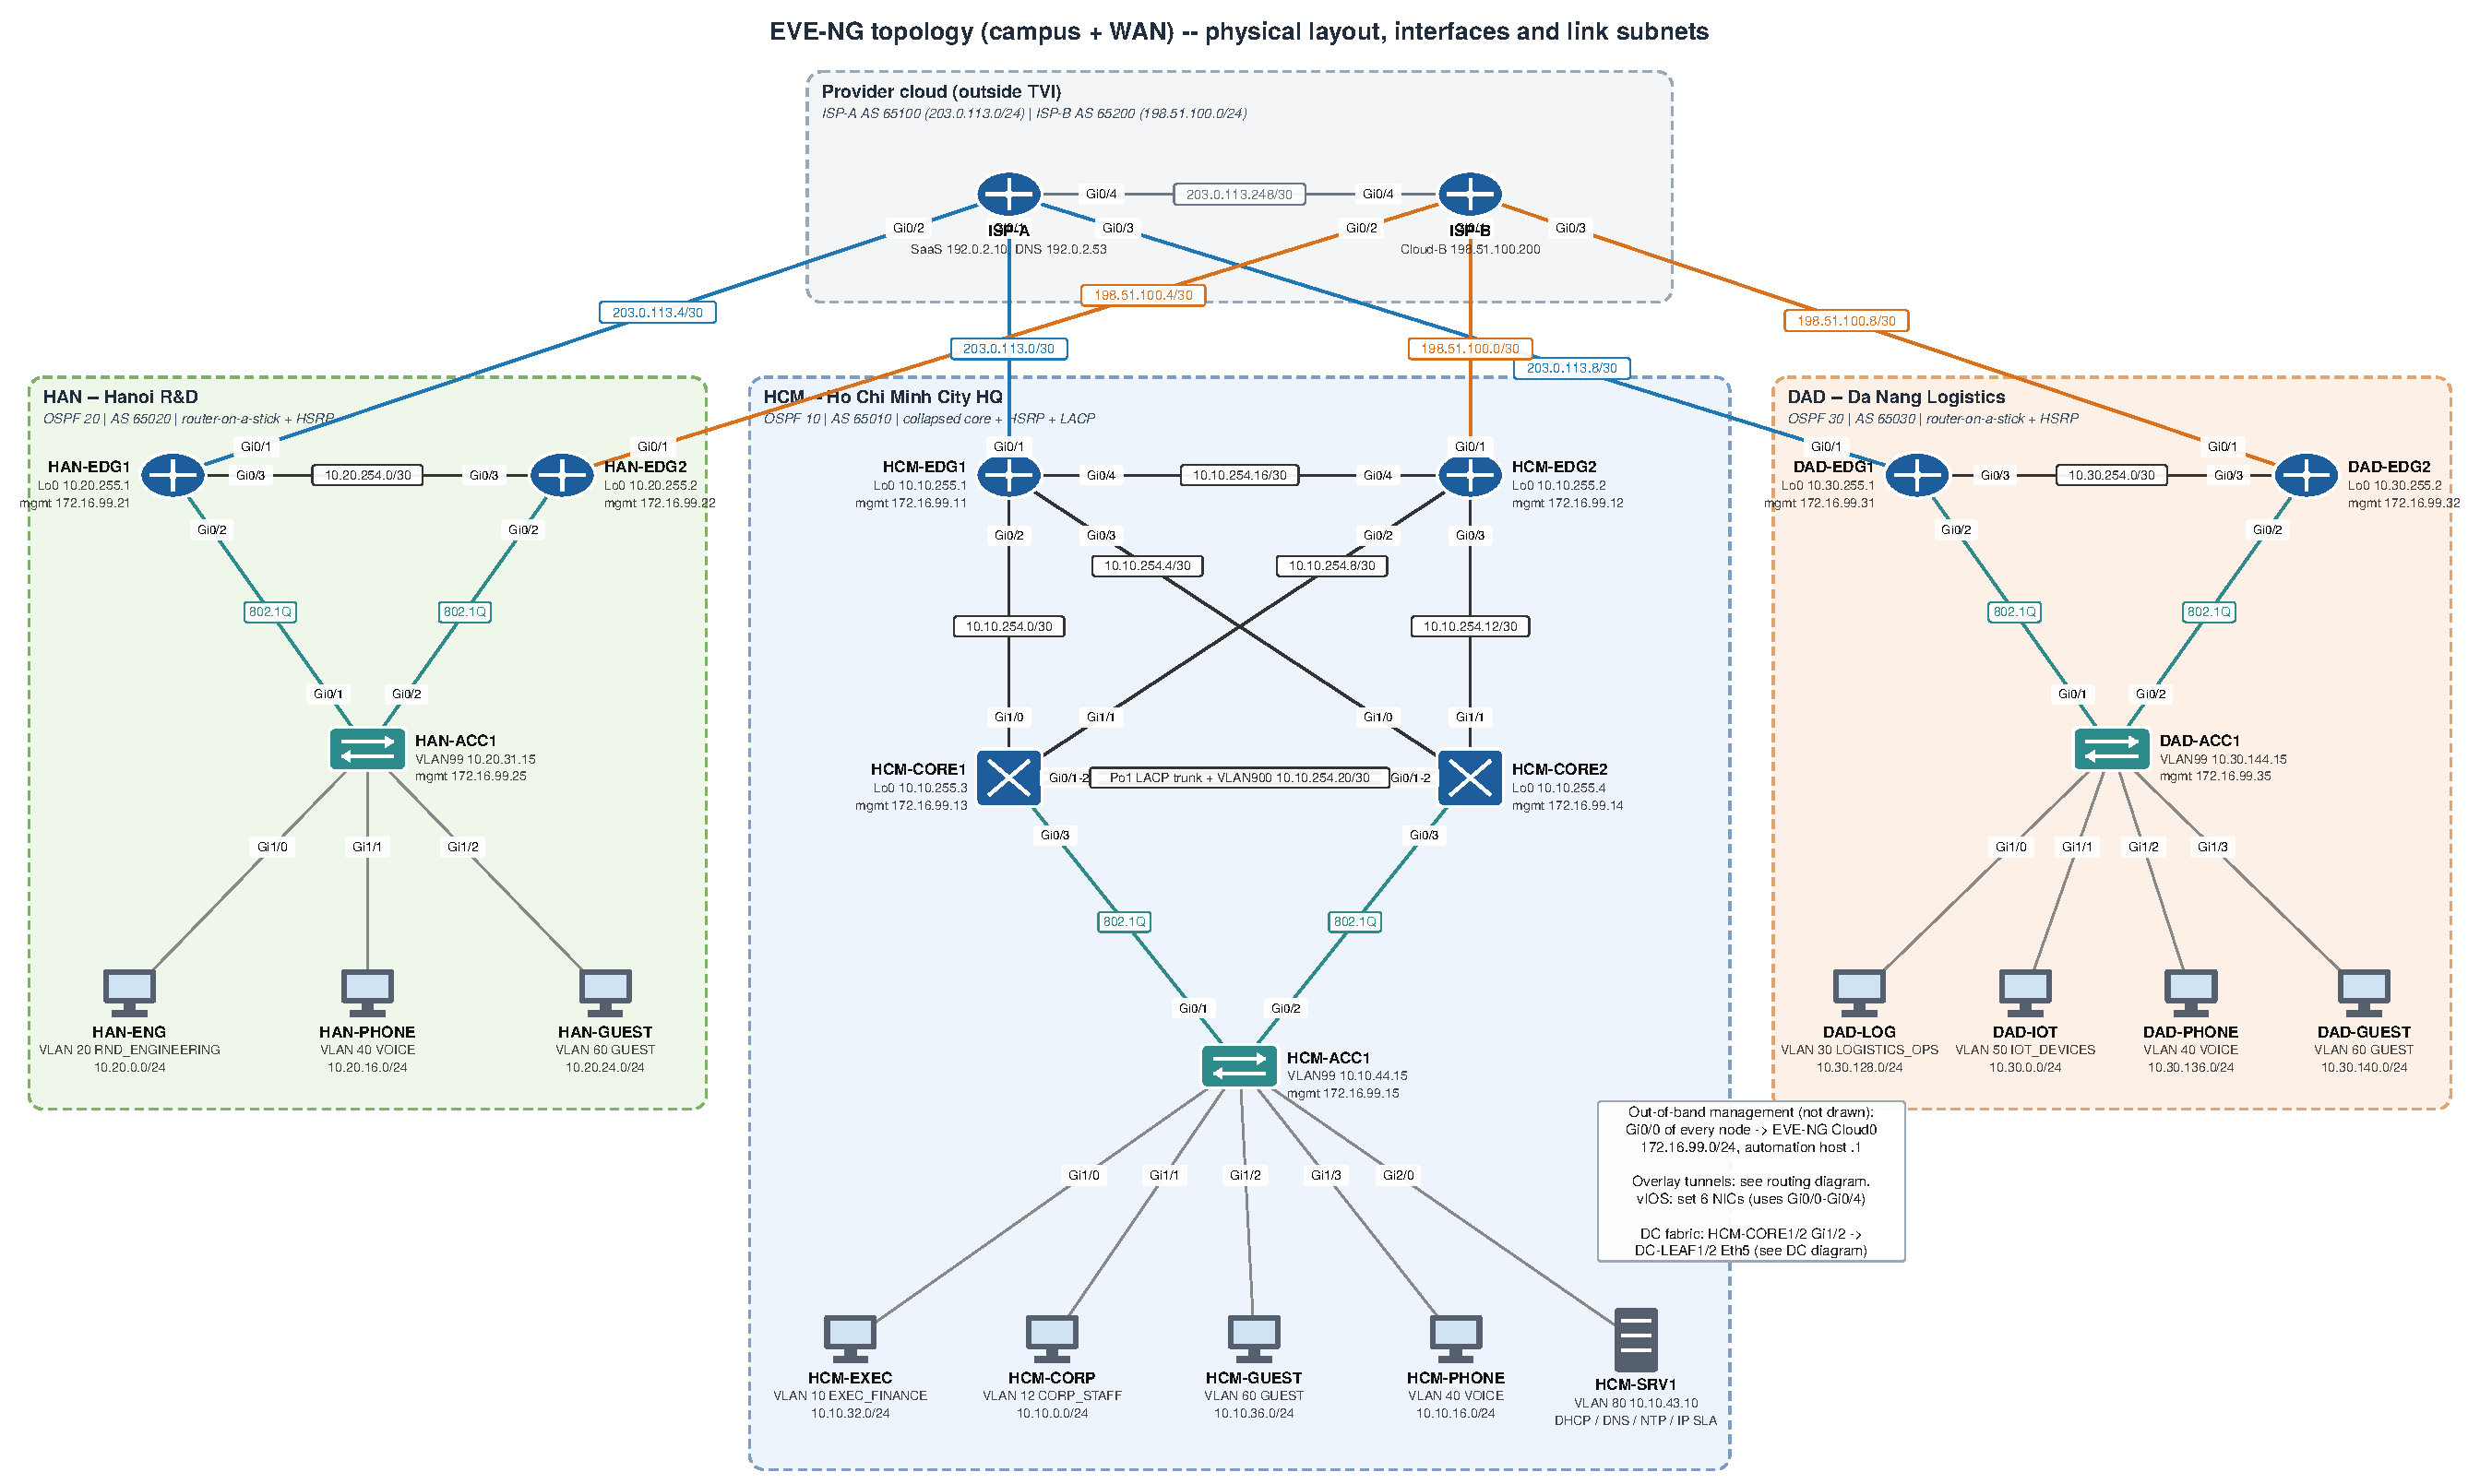
\includegraphics[width=\linewidth]{figures/02-labA-physical.pdf}
\caption{Lab A physical topology: interfaces, link subnets and VLAN placement}
\label{fig:physical}
\end{figure}

\subsection{Lab inventory and resource budget}

Table~\ref{tab:devices} lists every node with its image, loopback and out-of-band management address. All Cisco and Arista nodes connect their first interface (\texttt{Gi0/0}/\texttt{Management1}) to an EVE-NG \emph{Cloud0} network (172.16.99.0/24), which is how the automation host reaches them without depending on the production data plane. Lab A requires \ramA\,GB and Lab B \ramB\,GB of RAM, so each lab runs on its own on a 12\,GB host; they are demonstrated one after the other.

\begin{table}[H]
\centering\scriptsize
\caption{Lab node inventory (generated from the source of truth)}
\label{tab:devices}
\begin{tabularx}{\linewidth}{@{}l c l l l X l r@{}}
\toprule
\textbf{Node} & \textbf{Lab} & \textbf{Image} & \textbf{Role} & \textbf{Loopback0 / host IP} & \textbf{Loopback0 IPv6} & \textbf{OOB mgmt} & \textbf{MB}\\
\midrule
\tabin{generated/tab_devices.tex}
\bottomrule
\end{tabularx}
\end{table}

% ======================================================================== 4
\section{IP Addressing Strategy}
\label{sec:ip}

\subsection{Principles}

The plan follows four rules. First, \emph{one summary per site}: HCM, HAN and DAD own 10.10.0.0/16, 10.20.0.0/16 and 10.30.0.0/16, and 2001:db8:a010::/48, 2001:db8:a020::/48 and 2001:db8:a030::/48 respectively, so each site is advertised to the overlay as exactly one IPv4 and one IPv6 prefix. Second, \emph{VLSM by function}: inside each site, a pool is allocated per function and per VLAN, largest first and sized for 2030 demand, which avoids both overlap and the waste of uniform /16s. Third, \emph{bounded broadcast domains}: every pool is consumed in /24 access blocks, so no VLAN ever exceeds 254 hosts -- a deliberate answer to the broadcast storms of the legacy network. Fourth, \emph{readability}: the second octet identifies the site, the IPv6 fourth hextet encodes the VLAN and the access block (VVBB), loopbacks live in x.x.255.0/24 and point-to-point links in x.x.254.0/24.

\begin{table}[H]
\centering\small
\caption{Site summaries, routing identifiers and user growth}
\label{tab:sites}
\begin{tabular}{@{}l l l l r r r r@{}}
\toprule
\textbf{Site} & \textbf{Name} & \textbf{IPv4} & \textbf{IPv6} & \textbf{AS} & \textbf{OSPF} & \textbf{Users} & \textbf{2030}\\
\midrule
\tabin{generated/tab_sites.tex}
\bottomrule
\end{tabular}
\end{table}

\subsection{IPv4 VLSM allocation}

Table~\ref{tab:pools} shows the complete allocation. The ``Demand 2030'' column is an assumption derived from the brief: the user base grows from 4,000 to 10,000, phones are provisioned for roughly 70\,\% of staff, and the Da Nang IoT estate grows from 10,000 to 25,000 devices as warehouse automation expands. Every pool covers its 2030 demand, and large ranges (for example 10.10.64.0--10.10.127.255 and 10.30.146.0--10.30.253.255) remain unallocated for functions that do not yet exist.

{\footnotesize\setlength{\tabcolsep}{4pt}
\begin{longtable}{@{}l l l r r r p{4.6cm}@{}}
\caption{IPv4 VLSM pools per site, sized for 2030}\label{tab:pools}\\
\toprule
\textbf{Site} & \textbf{VLAN / use} & \textbf{Pool} & \textbf{Usable} & \textbf{2030} & \textbf{Util.} & \textbf{Notes}\\
\midrule\endfirsthead
\toprule
\textbf{Site} & \textbf{VLAN / use} & \textbf{Pool} & \textbf{Usable} & \textbf{2030} & \textbf{Util.} & \textbf{Notes}\\
\midrule\endhead
\tabin{generated/tab_pools.tex}
\bottomrule
\end{longtable}}

The overlay uses 10.0.0.0/24 (/30 per tunnel), and 10.0.64.0/18 is reserved for the ZTNA connector pool. Since the three sites consume only three of the 256 possible /16s in 10.0.0.0/8, a new site requires no change to existing prefixes or filters: the inbound BGP prefix-list already accepts any 10.x.0.0/16.

\subsection{Deployed subnets and gateways}

Table~\ref{tab:deployed} lists the subnets configured in the lab -- the first /24 access block of each pool. Every subnet has an HSRP virtual gateway at .1 (FE80::1 for IPv6), with the two physical gateways at .2 and .3.

\begin{table}[H]
\centering\scriptsize
\caption{Deployed gateway subnets in Lab A}
\label{tab:deployed}
\setlength{\tabcolsep}{3pt}
\begin{tabularx}{\linewidth}{@{}l r l l l l l X@{}}
\toprule
\textbf{Site} & \textbf{VLAN} & \textbf{Name} & \textbf{IPv4} & \textbf{IPv6 /64} & \textbf{HSRP active} & \textbf{DHCP} & \textbf{ACL}\\
\midrule
\tabin{generated/tab_deployed.tex}
\bottomrule
\end{tabularx}
\end{table}

\subsection{IPv6 hierarchy}

TVI's IPv6 allocation is 2001:db8:a000::/40, which contains 256 site /48s. Within a site, the fourth hextet is structured as \texttt{VVBB}: VV is the VLAN number written in decimal digits and BB the access-block number, so VLAN~20, block~01 in Hanoi is 2001:db8:a020:2001::/64 and can be recognised without a lookup table. The values fe01--fe06 are reserved for point-to-point links and ff00 for loopbacks (with the last octet of the IPv4 loopback as the interface identifier). Each /48 offers 65,536 /64s, enough for 99 blocks of every VLAN with room to spare. The guest VLANs are deliberately IPv4-only, since the guest service is Internet access and the lab carriers provide no IPv6 transit.

\subsection{Point-to-point links, tunnels and summarisation}

\begin{table}[H]
\centering\scriptsize
\caption{Point-to-point, carrier and overlay links}
\label{tab:links}
\begin{tabular}{@{}l l l l@{}}
\toprule
\textbf{Side A} & \textbf{Side B} & \textbf{IPv4} & \textbf{IPv6}\\
\midrule
\tabin{generated/tab_links.tex}
\bottomrule
\end{tabular}
\end{table}

Summarisation happens at the BGP edge: each edge router originates its site /16 and /48 from a discard (Null0) route with administrative distance 254, which keeps the summary stable even when individual subnets flap and prevents routing loops for unused addresses inside the block. The complete plan, with formulas for capacity and utilisation, is also provided as \texttt{ip-plan/TVI\_IP\_Plan.xlsx}.

% ======================================================================== 5
\section{Core Infrastructure and Technology Rationale}
\label{sec:core}

\subsection{Layer 2: VLANs, trunking, EtherChannel and spanning tree}
\label{sec:l2}

\begin{figure}[H]
\centering
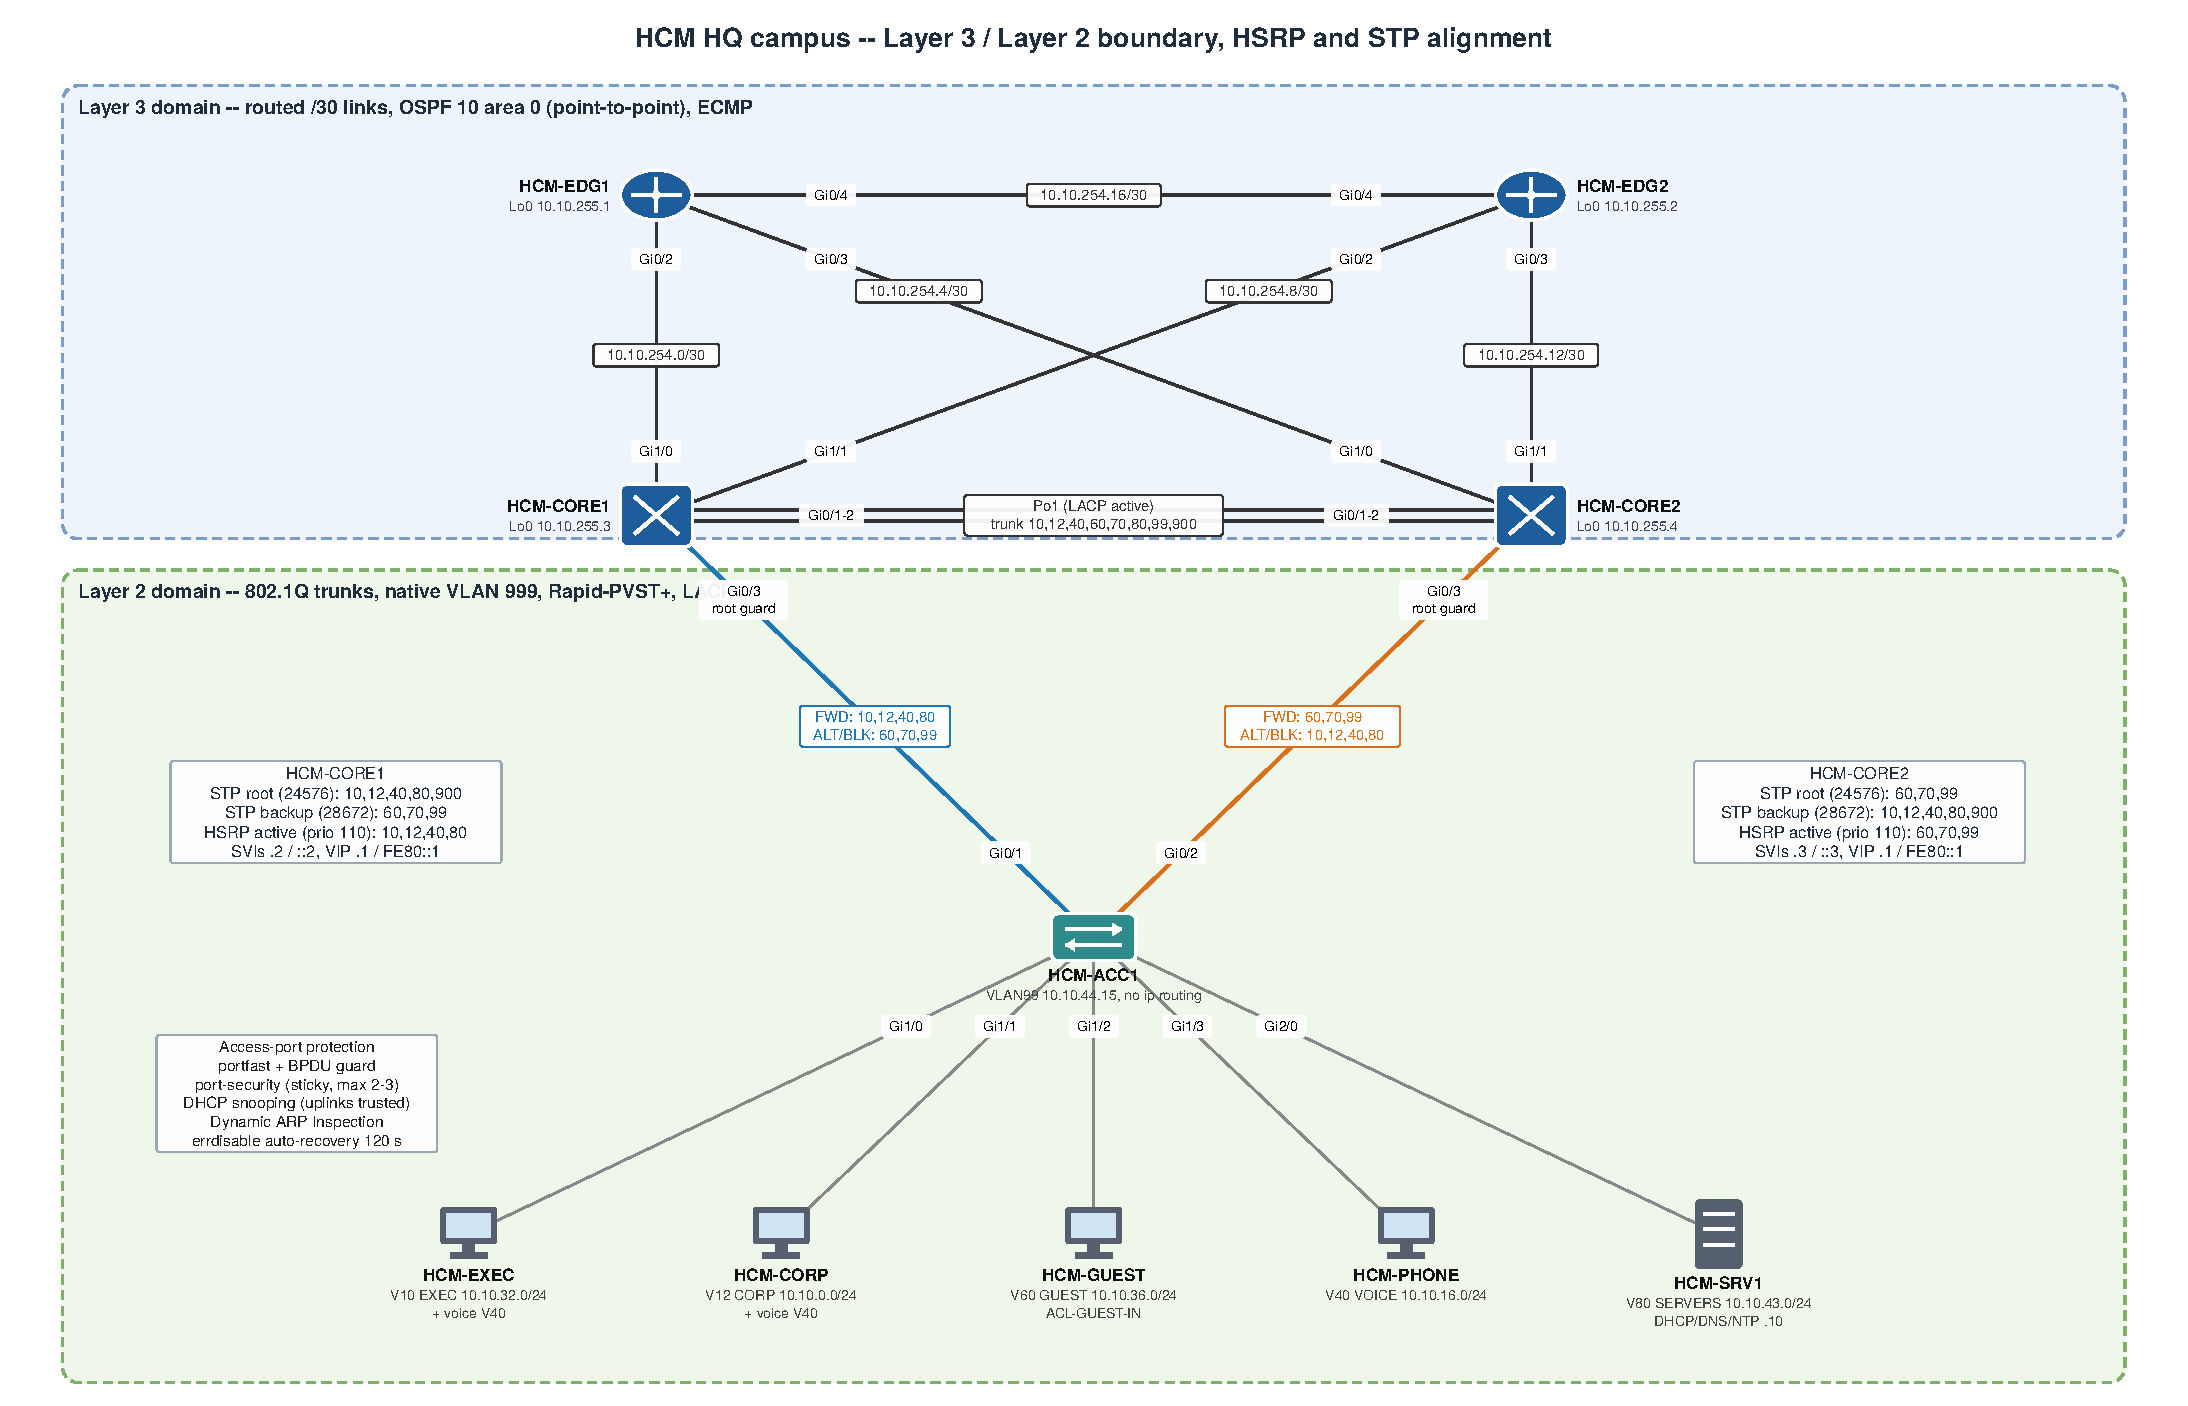
\includegraphics[width=0.92\linewidth]{figures/04-hcm-l2-l3.pdf}
\caption{HCM campus: Layer 3/Layer 2 boundary, HSRP and spanning-tree alignment}
\label{fig:hcm}
\end{figure}

\paragraph{VLANs and trunks.} VLAN identifiers are global (Table~\ref{tab:deployed}), which simplifies operations and automation. All trunks are static 802.1Q trunks with DTP disabled (\texttt{switchport nonegotiate}), an unused native VLAN 999 to defeat VLAN-hopping, and an explicit allowed list, so that a VLAN exists only where it is needed. VTP is set to transparent so that a misconfigured switch cannot delete VLANs across the campus; VLAN consistency is enforced by the automation instead (Section~\ref{sec:auto}).

\paragraph{EtherChannel.} The two HQ core switches are joined by Port-channel~1, two links negotiated with LACP (\texttt{mode active}). LACP was preferred to static bundling because it detects a mis-cabled or unidirectional member and removes it, and to PAgP because it is an IEEE standard (802.1AX). The bundle carries all user VLANs plus VLAN 900, a /30 transit used only for the OSPF adjacency between the cores. Losing one member halves the bandwidth but causes no topology change for STP or OSPF.

\lstinputlisting[caption={HCM-CORE1 -- LACP bundle to HCM-CORE2},label=lst:lacp]{generated/cfg_lacp.txt}

\paragraph{Spanning tree.} Rapid-PVST+ (802.1w per VLAN) provides sub-second convergence on point-to-point links. The root bridge is \emph{not} left to the lowest MAC address: HCM-CORE1 has priority 24576 for VLANs 10, 12, 40, 80 and 900 and 28672 for VLANs 60, 70 and 99; HCM-CORE2 has the opposite. Because the HSRP active gateway of each VLAN is the same switch as its STP root (Figure~\ref{fig:hcm}), traffic always takes the forwarding uplink directly to its gateway and never crosses the inter-core link, and the two uplinks of the access switch are both used, each for half of the VLANs. Root guard on the core downlinks prevents an access switch from ever becoming root, BPDU guard and PortFast protect edge ports, and loop guard protects against unidirectional links. MST would be preferred once the number of VLANs grows into the hundreds; for the present VLAN count, per-VLAN load balancing with Rapid-PVST+ is simpler to operate.

\lstinputlisting[caption={HCM-CORE1 -- deterministic root placement}]{generated/cfg_stp.txt}

\subsection{First-hop redundancy and IP services}
\label{sec:fhrp}

\paragraph{HSRP version 2.} Every gateway subnet has an HSRPv2 group for IPv4 (group = VLAN number) and one for IPv6 (group = 1000 + VLAN, virtual link-local FE80::1). HSRP was chosen over VRRP because both gateways are Cisco devices and HSRPv2 supports IPv6 groups with a fixed virtual link-local address, which lets every IPv6 host and server use the same next hop FE80::1 regardless of which router is active. Hello/hold timers of 1/3\,s bound failover to about three seconds; \texttt{preempt delay minimum 10} returns the role to the preferred router only after its routing protocols have converged, which avoids black-holing traffic after a reboot. Active roles are split between the two gateways for load sharing: at the branches, the EDG1 router serves data and management VLANs while EDG2 serves voice, IoT and guests, so data and voice leave the site on different carriers.

\lstinputlisting[caption={HCM-CORE1 -- dual-stack HSRPv2 gateway for the Executive VLAN}]{generated/cfg_hsrp.txt}

\paragraph{Centralised DHCP, DNS and NTP.} A single DHCP service at HQ (HCM-SRV1, 10.10.43.10) serves all twelve DHCP-enabled subnets of the three sites, as the brief requires. Every gateway relays requests with \texttt{ip helper-address}; the relay sets the \emph{giaddr} field to the gateway's own address, which the server uses to choose the pool. Because both HSRP peers relay, the server receives two copies of each request and the client accepts the first offer; this is the intended redundancy of the relay function. Excluded ranges (.1--.20) protect the gateway and static addresses. Guest pools hand out a public resolver and a 4-hour lease, corporate pools the internal DNS and a 1-day lease, and the AP pool carries DHCP option 43 with the controller address (Section~\ref{sec:wlan}). The same server is the internal DNS (with records for every device loopback and forwarding to the Internet resolver) and the NTP master to which every device is synchronised.

\lstinputlisting[caption={HCM-SRV1 -- a branch pool and the AP pool with option 43}]{generated/cfg_dhcp.txt}

\subsection{Underlay routing: OSPFv2 and OSPFv3}
\label{sec:ospf}

Each site runs its own OSPF domain (process 10, 20 or 30) for both IPv4 and IPv6 (OSPFv3), all in area 0. OSPF was chosen over EIGRP because it is an open standard that also runs on non-Cisco equipment such as the Arista data-centre fabric, converges quickly and supports IPv6 natively through OSPFv3. A single area per site is appropriate because each site contains only a handful of routers; a multi-area hierarchy would add ABR complexity without reducing any meaningful LSA load.

Three settings matter. All transit links use \texttt{ip ospf network point-to-point}, which removes the DR/BDR election and the associated delay on two-router segments. The reference bandwidth is raised to 100\,Gbps so that 1, 10 and 40\,GbE links receive distinct costs. Finally, \texttt{passive-interface default} with explicit exceptions ensures that adjacencies form only on infrastructure links: user VLANs are advertised but never accept an OSPF neighbour, which closes an obvious attack vector.

The underlay does not extend across the WAN. At HQ, the edge routers originate a default route (only while they hold one from their carrier) and redistribute the eBGP-learned remote-site summaries as external type-2 routes; the cores therefore see each remote /16 through both edges and load-share with ECMP. At the branches, the edge routers are themselves the gateways and need no redistribution.

\lstinputlisting[caption={HCM-EDG1 -- OSPFv2/v3 underlay and controlled redistribution}]{generated/cfg_ospf.txt}

\subsection{Overlay routing and WAN edge: BGP over GRE/IPsec}
\label{sec:overlay}

\begin{figure}[H]
\centering
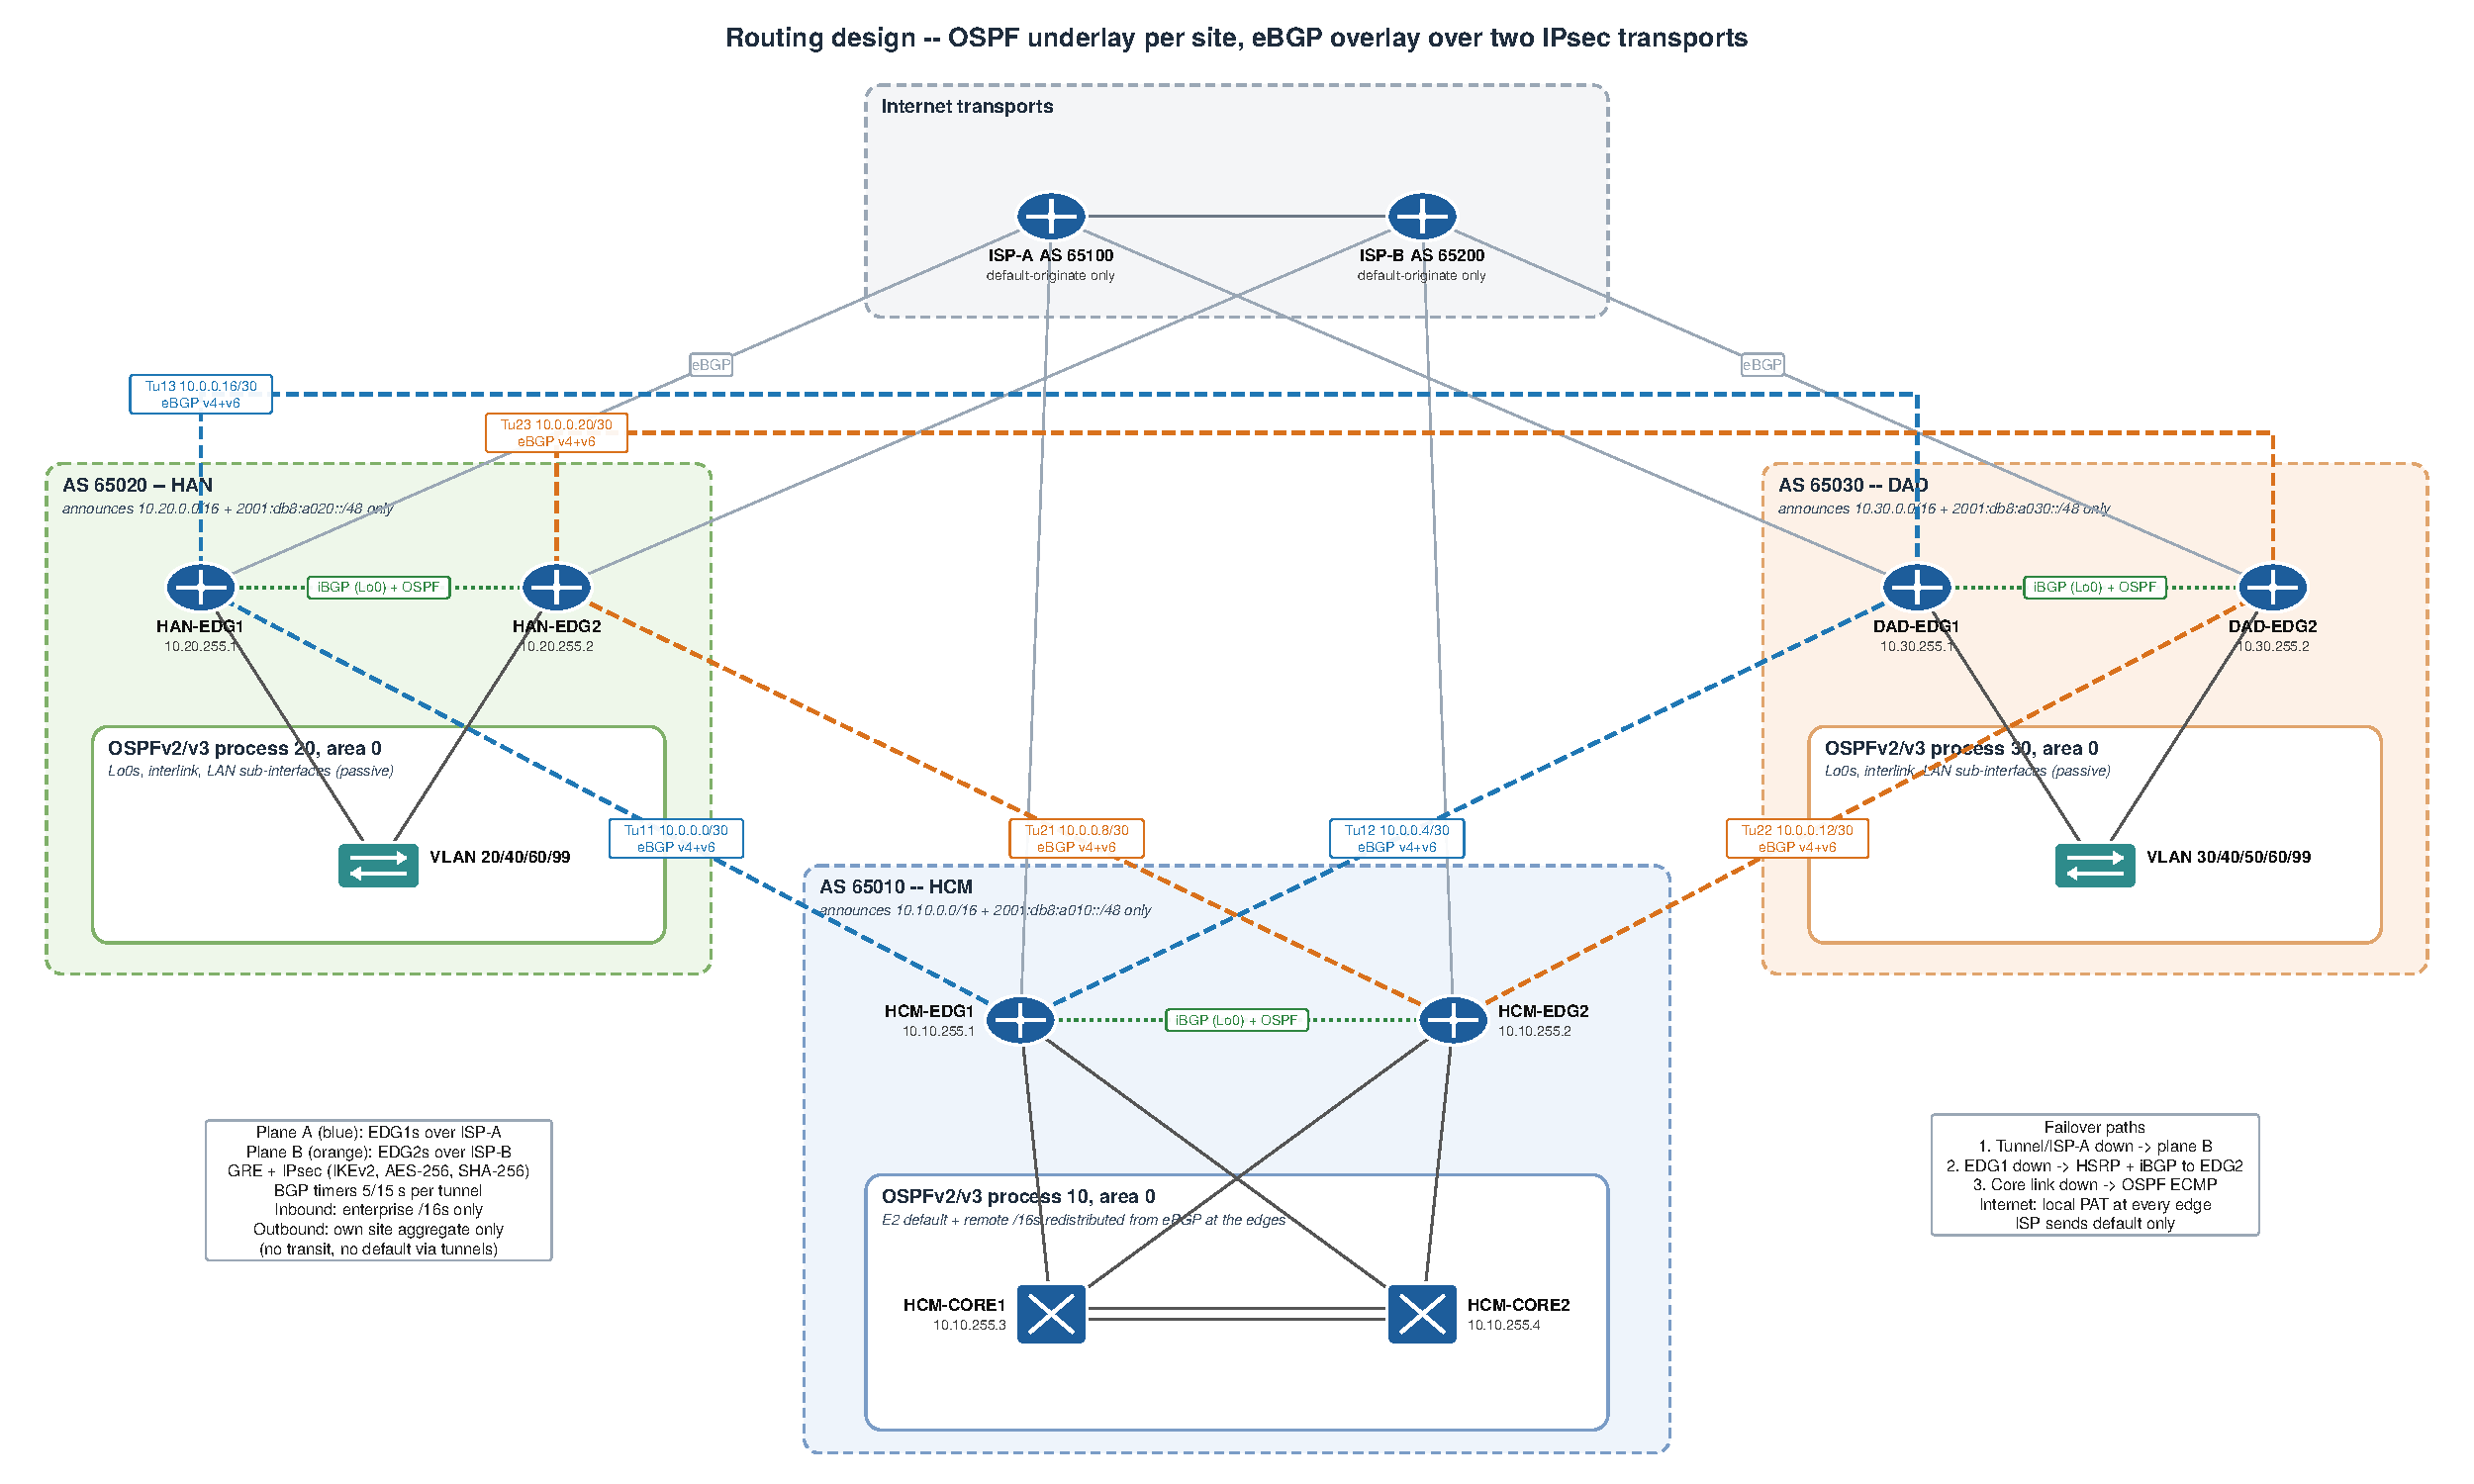
\includegraphics[width=\linewidth]{figures/03-routing-overlay.pdf}
\caption{Routing domains: per-site OSPF underlay, eBGP overlay on two transport planes}
\label{fig:routing}
\end{figure}

\paragraph{SD-WAN emulation.} A commercial SD-WAN product builds encrypted tunnels across every available transport and chooses between them per application. The lab reproduces the essential mechanics with standard protocols (Figure~\ref{fig:routing}). On each carrier, the three sites are connected by a full mesh of GRE tunnels protected by IPsec, giving two independent \emph{planes}: plane A (Tunnels 11--13 between the EDG1 routers over ISP-A) and plane B (Tunnels 21--23 between the EDG2 routers over ISP-B). A full mesh rather than hub-and-spoke means Hanoi and Da Nang communicate directly, which removes the HQ hairpin that the brief identifies as a cause of latency. GRE is used inside IPsec, rather than a pure IPsec VTI, because GRE carries IPv4 and IPv6 in the same tunnel and therefore supports dual-stack BGP and multicast-based protocols if required later.

\lstinputlisting[caption={HCM-EDG1 -- IKEv2/IPsec profile protecting the GRE overlay}]{generated/cfg_ipsec.txt}
\lstinputlisting[caption={HCM-EDG1 -- overlay tunnel on plane A}]{generated/cfg_tunnel.txt}

IKEv2 with AES-256-CBC, SHA-256 and Diffie-Hellman group 14 protects the tunnels, satisfying the executive requirement for encrypted traffic on every inter-site path. Transport mode avoids a redundant second IP header because GRE already provides one, and the tunnel MTU (1400) with TCP MSS clamping (1360) prevents fragmentation of the encapsulated packets.

\paragraph{BGP design.} Each site is a private autonomous system (65010, 65020, 65030), the two edges of a site run iBGP between their loopbacks, and every tunnel carries one eBGP session for IPv4 and one for IPv6 (MP-BGP address families). eBGP between sites was preferred to a single iBGP domain because it needs no full mesh or route reflector across the WAN, because the AS path provides natural loop prevention, and because it gives each site an explicit routing policy boundary. The policy is strict:
\begin{itemize}
\item towards the carriers, nothing is advertised (\texttt{PL-DENY-ALL}) and only a default route is accepted (\texttt{PL-DEFAULT-ONLY}), so TVI's private space can never leak to the Internet;
\item on the overlay, each site advertises only its own /16 and /48 (\texttt{PL-SITE-OUT}) and accepts only enterprise /16--/24 prefixes (\texttt{PL-ENTERPRISE-IN}); the default route is never exchanged between sites, which keeps Internet traffic local, and transit through a third site is impossible;
\item iBGP between the two edges of a site uses \texttt{next-hop-self}, so each edge can reach the other plane through its partner when its own tunnels or carrier fail.
\end{itemize}

\lstinputlisting[caption={HCM-EDG1 -- BGP neighbours and IPv4 policy (IPv6 family analogous)}]{generated/cfg_bgp.txt}

BGP keepalive/hold timers on the tunnels are reduced to 5/15\,s, bounding the detection of a failed tunnel or carrier to 15 seconds; BFD would reduce this further on hardware platforms. Path selection follows standard BGP rules: an edge prefers its own eBGP-learned path (shorter AS path than the iBGP alternative), so each plane carries the traffic of the gateways that use it, and the other plane takes over automatically.

\paragraph{Local Internet breakout and NAT.} Each edge translates its own site's traffic to the address of its carrier interface (PAT overload). The NAT access list explicitly denies 10.0.0.0/8-to-10.0.0.0/8 traffic, so site-to-site flows are never translated, and only the carrier-facing interface is \texttt{ip nat outside}. Branches therefore reach SaaS applications in one hop to their carrier instead of crossing the WAN to HQ.

\lstinputlisting[caption={Edge PAT -- Internet-bound traffic only}]{generated/cfg_nat.txt}

\paragraph{Interaction of underlay and overlay.} The underlay and the overlay interact at exactly two points, both on the edge routers. First, the overlay depends on the underlay for reachability of the iBGP loopbacks and on the carrier default route for the tunnel endpoints; because the tunnel destination is resolved only through the carrier default (and never through a route learned over a tunnel, which the prefix-lists exclude), recursive routing loops cannot occur. Second, the overlay feeds the underlay: HQ redistributes only remote-site summaries, and only eBGP-learned ones, into OSPF. If HCM-EDG1 loses its tunnels, its eBGP routes disappear, it stops redistributing them, and the cores immediately shift to HCM-EDG2 without any manual action.

\subsection{Data-centre fabric: EVPN-VXLAN (Lab B)}
\label{sec:evpn}

\begin{figure}[H]
\centering
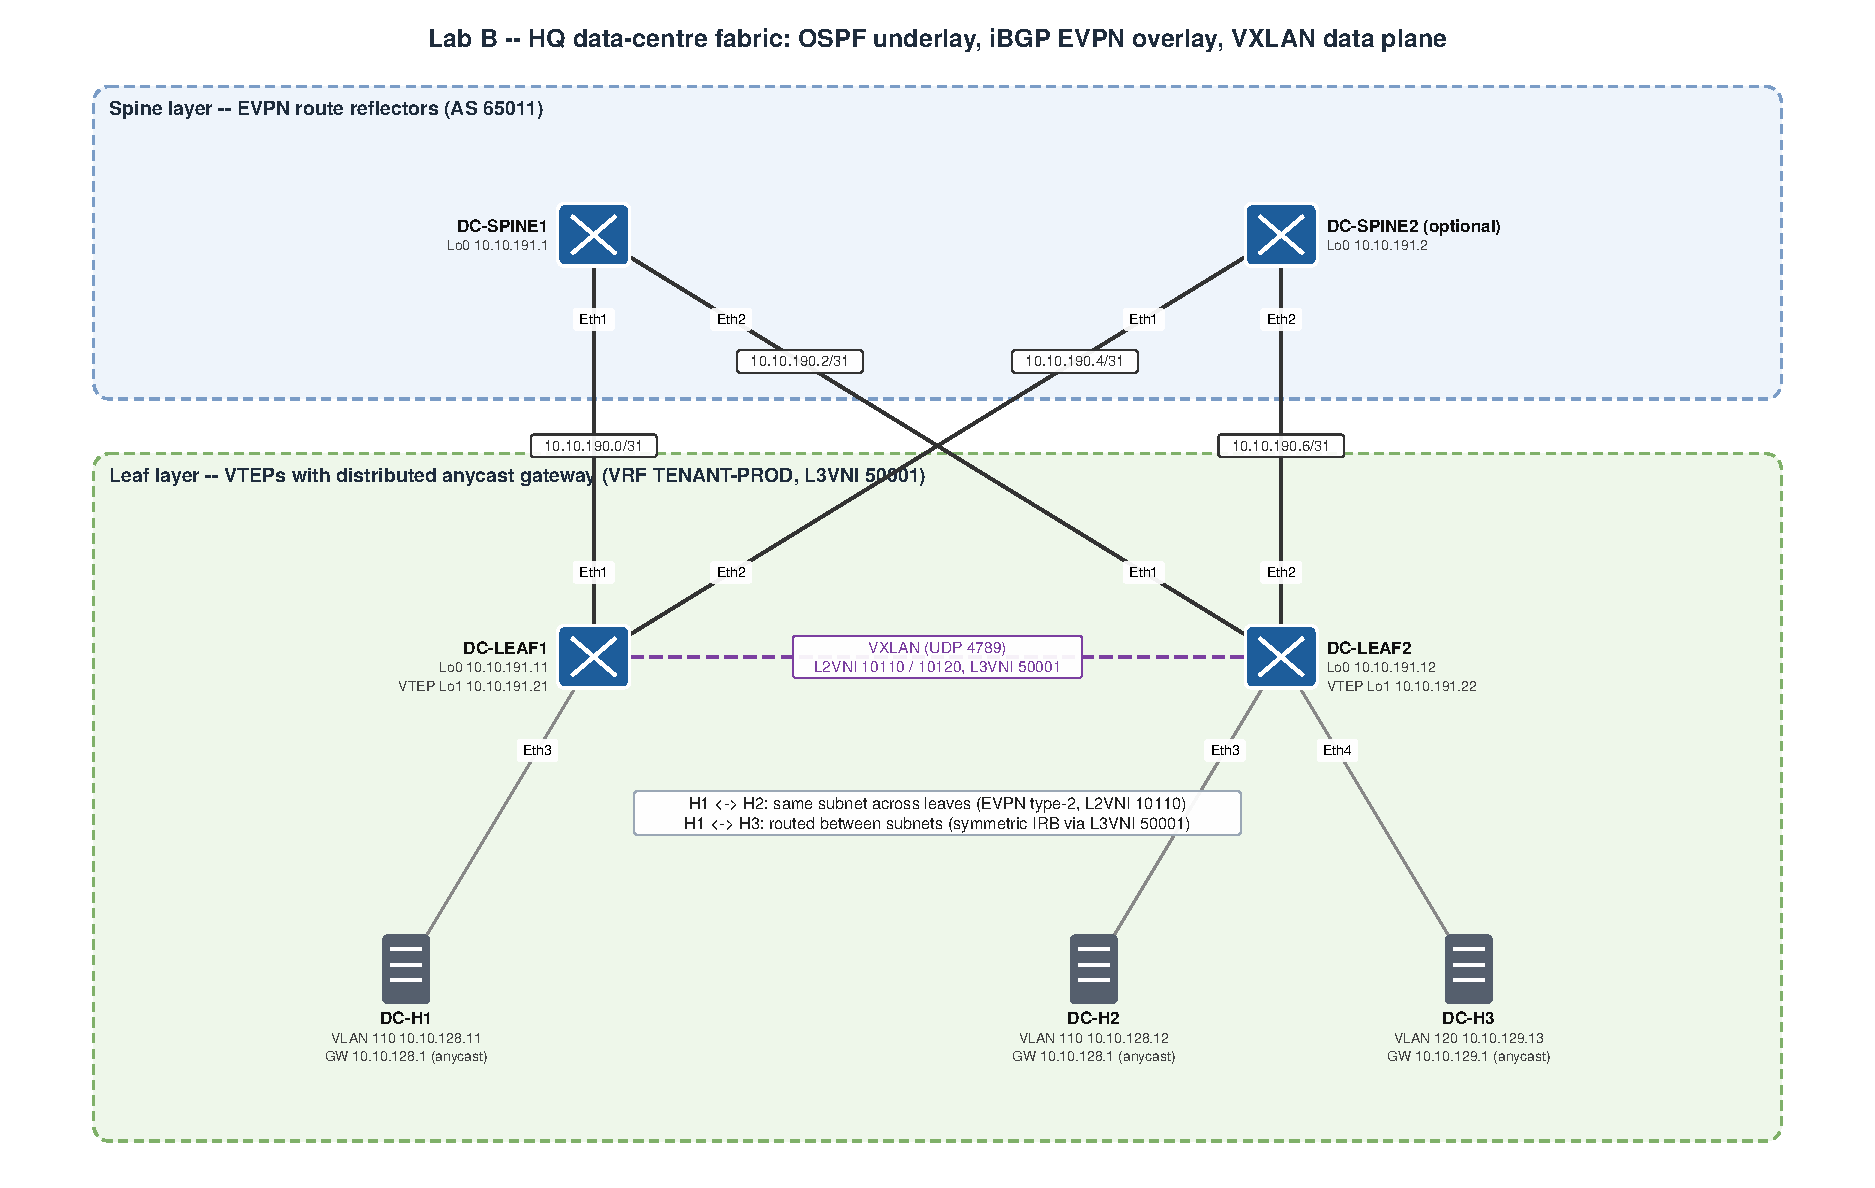
\includegraphics[width=0.85\linewidth]{figures/05-dc-evpn-fabric.pdf}
\caption{HQ data-centre fabric: spine-leaf with EVPN control plane and VXLAN data plane}
\label{fig:dc}
\end{figure}

The HQ data centre and the Hanoi AI lab require large east-west bandwidth and workload mobility, which a traditional Layer~2 design with spanning tree cannot provide at scale. A spine-leaf fabric gives every leaf an equal-cost path to every other leaf through any spine, and VXLAN extends Layer~2 segments over this routed fabric without spanning tree. EVPN (RFC~7432/8365) replaces flood-and-learn with a BGP control plane: leaves advertise MAC/IP bindings (route type 2) and subnets (type 5), which suppresses unnecessary flooding and supports multi-tenancy with VRFs.

The fabric in Lab B (Figure~\ref{fig:dc}) uses OSPF on /31 point-to-point links as the underlay (matching the brief's OSPF-underlay/BGP-overlay model), iBGP EVPN with the spines as route reflectors, and a distributed anycast gateway (10.10.128.1 and 10.10.129.1 on every leaf). VLAN 110 and VLAN 120 map to L2VNIs 10110 and 10120; routing between them uses symmetric IRB through L3VNI 50001 in VRF TENANT-PROD. In production, a pair of border leaves would connect the fabric to the HQ cores and the fabric's VRF would be advertised into OSPF; this connection is omitted from the lab only because of the RAM budget.

\lstinputlisting[caption={DC-LEAF1 -- VXLAN mapping and EVPN configuration}]{generated/cfg_evpn_leaf.txt}

\subsection{Wireless: WLC and CAPWAP}
\label{sec:wlan}

Wireless is controller-based. Access points live in VLAN~70 (a /23 at Da Nang for the dense warehouse deployment), obtain an address from the central DHCP server and learn the controller address 10.10.43.20 from DHCP option~43 (sub-option 0xF1, value \texttt{0a0a2b14}). They then build CAPWAP tunnels (UDP 5246 control, 5247 data) to the controller. The controller authenticates corporate users with 802.1X and assigns their VLAN dynamically from RADIUS attributes, so an executive and a guest associated to the same SSID infrastructure still land in different VLANs and policies. For the Da Nang AGVs and scanners, Wi-Fi~6/7 with 802.11r/k/v fast roaming and a dedicated 5/6\,GHz SSID provides the low and predictable latency required by autonomous vehicles. Because a virtual controller (Cisco C9800-CL) needs more memory than the lab host has, the WLC is a design element: the switch-side configuration (AP VLAN, DHCP option 43, QoS) is implemented, the controller is not.

\subsection{High availability analysis}
\label{sec:ha}

\begin{table}[H]
\centering\small
\caption{Single-failure analysis}
\label{tab:spof}
\begin{tabularx}{\linewidth}{@{}p{3.6cm}X p{2.6cm}@{}}
\toprule
\textbf{Failure} & \textbf{Recovery mechanism} & \textbf{Expected impact}\\
\midrule
One LACP member link & Remaining member keeps Port-channel~1 up & None (bandwidth halved)\\
Core--edge link at HQ & OSPF removes the link; ECMP via the other path & $<$1\,s\\
HQ core switch & HSRP standby becomes active; RSTP unblocks the alternate uplink & 3\,s\\
Branch edge router & HSRP failover of its VLANs; partner forwards via its own plane & 3\,s\\
Carrier or tunnel (one plane) & BGP hold timer expires; traffic uses the other plane via iBGP & $\le$15\,s\\
Access switch & Not redundant in the lab; dual-homed endpoints / stacks in production & site of one closet\\
DHCP server & Leases persist (1 day); a second server with split scopes in production & none short-term\\
\bottomrule
\end{tabularx}
\end{table}

Four-nines availability allows 52.6 minutes of downtime per year. With redundant gateways, links and carriers, no single failure in Table~\ref{tab:spof} takes a service down for more than seconds; the remaining exposure is concentrated in the access layer, which production mitigates with stacked access switches and dual-homed APs, and in maintenance windows, which the redundant pairs allow to be performed one device at a time.

% ======================================================================== 6
\section{Security, QoS and Automation Strategy}
\label{sec:secqos}

\subsection{Segmentation policy}
\label{sec:sec}

Security is layered. Table~\ref{tab:matrix} is the intended communication matrix; the ACLs, the firewall and the routing policy below enforce it.

\begin{table}[H]
\centering\small
\caption{Segmentation matrix (row = source, column = destination)}
\label{tab:matrix}
\footnotesize\setlength{\tabcolsep}{5pt}
\begin{tabular}{@{}l c c c c c c c@{}}
\toprule
 & \textbf{Exec} & \textbf{Staff} & \textbf{Voice} & \textbf{IoT} & \textbf{Servers} & \textbf{Guest} & \textbf{Internet}\\
\midrule
Exec (V10) & -- & \checkmark & \checkmark & $\times$ & \checkmark & $\times$ & \checkmark\\
Staff (V12/20/30) & reply only & \checkmark & \checkmark & $\times$ & \checkmark & $\times$ & \checkmark\\
Voice (V40) & reply only & \checkmark & \checkmark & $\times$ & \checkmark & $\times$ & \checkmark\\
IoT (V50) & $\times$ & $\times$ & $\times$ & $\times$ & MQTT, DNS, NTP & $\times$ & IoT hub only\\
Servers / MGMT & \checkmark & \checkmark & \checkmark & \checkmark & \checkmark & $\times$ & \checkmark\\
Guest (V60) & $\times$ & $\times$ & $\times$ & $\times$ & DHCP only & $\times$ & \checkmark\\
\bottomrule
\end{tabular}
\end{table}

\paragraph{Guest isolation.} Applied inbound on every guest gateway, \texttt{ACL-GUEST-IN} permits DHCP, then denies every RFC~1918 destination and permits the rest. Because it is stateless and inbound, it also blocks replies from guests to internal hosts, so isolation holds in both directions.

\lstinputlisting[caption={ACL-GUEST-IN (all three sites)}]{generated/cfg_acl_guest.txt}

\paragraph{IoT micro-segmentation.} Warehouse devices are the least trustworthy endpoints on the network. \texttt{ACL-IOT-IN} allows only DHCP, DNS and NTP to the central server, MQTT (1883/8883) to the IoT platform in the HQ server VLAN, and MQTT over TLS to the cloud IoT hub; everything else is dropped and logged. An equivalent IPv6 ACL permits neighbour discovery explicitly, since an explicit \texttt{deny ipv6 any any} would otherwise override the implicit ND entries.

\lstinputlisting[caption={ACL-IOT-IN on the Da Nang IoT gateway}]{generated/cfg_acl_iot.txt}

\paragraph{Executive protection.} Executives initiate connections freely, but other internal subnets may only send replies (TCP \texttt{established} and ICMP replies) into VLAN 10; only the server and management subnets may open new sessions. The ACL is applied \emph{outbound} on the executive SVI of both cores, so it covers traffic from every site regardless of path, and an IPv6 twin applies the same logic.

\lstinputlisting[caption={ACL-EXEC-PROTECT (outbound on Vlan10)}]{generated/cfg_acl_exec.txt}

\paragraph{Zone-based firewall at the edge.} Each edge router is a stateful firewall with two zones (Listing~\ref{lst:zbf}). The INSIDE zone contains LAN interfaces, the edge interlink and the overlay tunnels; the OUTSIDE zone contains the carrier interface. Traffic from INSIDE to OUTSIDE is inspected, so replies are admitted dynamically and nothing else enters. Traffic from the carrier to the router itself (the \emph{self} zone) is restricted to the control plane that must reach it: IKE (UDP 500/4500), ESP, GRE, BGP and ICMP. The overlay terminates inside the router, so decrypted site-to-site traffic appears on a Tunnel interface in the INSIDE zone and is governed by the ACLs above rather than by the Internet policy.

\lstinputlisting[caption={Zone-based firewall policy on every edge},label=lst:zbf]{generated/cfg_zbf.txt}

\paragraph{Layer 2 security.} Access switches enable DHCP snooping on every user VLAN, with only the uplinks trusted, so a rogue DHCP server on an access port is blocked; untrusted ports are rate-limited to 15 DHCP packets per second. Dynamic ARP Inspection validates ARP packets against the snooping bindings and drops spoofed replies, preventing man-in-the-middle attacks on the gateway. Port security limits each port to two or three MAC addresses (PC and phone) with sticky learning, and BPDU guard shuts any port on which a switch appears; error-disabled ports recover automatically after two minutes. Option 82 insertion is disabled because the relay function is on the gateways, not on the access switch.

\lstinputlisting[caption={DAD-ACC1 -- snooping, DAI and a protected IoT access port}]{generated/cfg_l2sec.txt}

\paragraph{Management plane.} SSH version 2 is the only remote access method, restricted by \texttt{ACL-MGMT-VTY} to the out-of-band network and the three management VLANs; local AAA, login rate limiting (\texttt{login block-for}), centralised syslog and NTP are enforced by the automation baseline.

\subsection{Zero Trust and SASE for the remote workforce}
\label{sec:ztna}

The legacy remote-access VPN placed a remote laptop on the internal network, which contradicts the segmentation above. The design replaces it with ZTNA delivered by a SASE provider, following NIST SP~800-207. Remote users authenticate to the SASE PoP with corporate identity and MFA; the PoP checks device posture and grants access to individual applications, never to a subnet. Lightweight connectors in the HQ server VLAN and the Hanoi AI-lab segment establish outbound-only connections to the PoP, so no inbound port is opened at the TVI edges, and the address pool 10.0.64.0/18 is reserved for connector-sourced traffic so that internal ACLs can still identify it. The same PoP provides a secure web gateway, CASB and firewall-as-a-service for remote users' Internet traffic. In the lab this component is documented but not emulated, since it is a cloud service rather than a device that EVE-NG can run.

\subsection{Quality of Service}
\label{sec:qos}

\begin{table}[H]
\centering\small
\caption{QoS classes on the WAN edge}
\label{tab:qos}
\begin{tabular}{@{}l l l l@{}}
\toprule
\textbf{Class} & \textbf{Classification at ingress} & \textbf{Marking} & \textbf{WAN egress treatment}\\
\midrule
Voice media & UDP 16384--32767 (RTP) from 10.0.0.0/8 & EF (46) & LLQ, strict priority 30\,\%\\
Call signalling & SIP UDP/TCP 5060--5061 & CS3 (24) & CBWFQ 5\,\%\\
Business-critical & Executive and site-admin subnets & AF31 (26) & CBWFQ 25\,\%\\
Default & everything else & 0 & fair-queue\\
\bottomrule
\end{tabular}
\end{table}

The QoS model follows RFC~4594. Classification and marking happen once, at the trust boundary where traffic enters the WAN edge from the LAN (\texttt{PM-LAN-MARK-IN}); anything not recognised is re-marked to 0, so an endpoint cannot obtain priority by marking its own packets. In production the trust boundary moves to the access port with a trusted IP phone; IOSvL2 does not support MQC on access ports, which is why the lab marks at the edge. On each carrier interface, a hierarchical policy shapes traffic to the contracted 50\,Mbps -- creating a queue that the router controls instead of the carrier -- and within it gives voice a strict-priority queue that is policed to 30\,\% so that it can never starve other classes. Because GRE and IPsec copy the inner DSCP to the outer header, the egress policy classifies encrypted tunnel traffic correctly; \texttt{qos pre-classify} is enabled on the tunnels as well.

\lstinputlisting[caption={Marking and hierarchical LLQ policy on the WAN edges}]{generated/cfg_qos.txt}

\paragraph{Simulated VoIP.} HCM-SRV1 generates G.711 voice streams with IP SLA \texttt{udp-jitter} probes towards responders on the HAN and DAD edges, marked EF. These probes provide traffic for the voice class counters and report the jitter, loss and MOS that a real call would experience.

\lstinputlisting[caption={HCM-SRV1 -- G.711 voice probe to Hanoi}]{generated/cfg_ipsla.txt}

\subsection{Network automation}
\label{sec:auto}

Automation is organised in two layers, both included in the submission.

\paragraph{Source of truth and configuration rendering.} Every site, VLAN, subnet, link, tunnel and AS number is defined once in \texttt{tools/sot.py}. Rendering scripts produce all eighteen device configurations, the IP plan (Excel and Markdown), the automation inventory, the diagrams and the tables in this report. A validation script (\texttt{tools/validate.py}) then checks the rendered configurations -- not the source data -- for 17 properties, including absence of duplicate addresses, matching subnets on both ends of every link, symmetric tunnels, bidirectional BGP sessions with correct AS numbers, consistent HSRP groups, STP root/HSRP alignment, defined ACLs and policy maps, and VLAN consistency on trunks. A deliberately broken configuration was used to confirm that the validator reports the errors.

\paragraph{Day-1 provisioning with Python and Netmiko.} \texttt{automation/tvi\_auto.py} fulfils the three Step~9 requirements:
\begin{enumerate}
\item \emph{Inventory and credentials.} Devices, management addresses, device types and roles are read from \texttt{inventory.yaml}; the payload comes from \texttt{vars/baseline.yaml} and \texttt{vars/vlans.yaml}. Credentials are read from the environment variables \texttt{TVI\_SSH\_USER} and \texttt{TVI\_SSH\_PASS} or requested interactively with \texttt{getpass}; neither the script nor the inventory contains a password, and a unit test enforces this.
\item \emph{Baseline and VLAN provisioning.} For every managed IOS node the script builds the baseline (AAA, NTP, syslog, banner, login hardening); for core and access switches it adds the standard VLANs 10 EXEC\_FINANCE, 20 RND\_ENGINEERING, 30 LOGISTICS\_OPS and 99 MANAGEMENT, plus any site-specific VLANs in the payload. Configuration is pushed with \texttt{send\_config\_set} using an error pattern, so a rejected command raises an exception instead of passing silently, and the result is saved with \texttt{write memory}.
\item \emph{State capture and backup.} Before and after the change, \texttt{show running-config} and \texttt{show ip interface brief} are saved in the \texttt{backups/} directory as \texttt{<hostname>\_<timestamp>\_backup.cfg} (plus an \texttt{\_ipbrief.txt} file), and a unified diff of the two configurations is written for review. Every success and every exception (timeout, authentication failure, rejected command) is logged to \texttt{logs/automation.log}.
\end{enumerate}

Beyond the minimum, the script verifies compliance after the push (each VLAN exists with the correct name), collects protocol telemetry (OSPF adjacencies, BGP sessions, HSRP states, LACP members, IKEv2 SAs) into JSON, works on several devices in parallel, can be restricted by site, role or host, and has a dry-run mode that prints the payload without connecting. Eight offline tests with a simulated device exercise the full workflow and the error paths; one of them found and fixed a real defect in which pre- and post-change backups written in the same second overwrote each other.

\begin{lstlisting}[caption={Typical automation runs},language=bash]
export TVI_SSH_USER=tviadmin            # password is prompted, never stored
python3 tvi_auto.py --dry-run --site HAN          # preview payload
python3 tvi_auto.py --task all                    # backup -> push -> backup -> diff -> verify
python3 tvi_auto.py --task telemetry --role edge  # OSPF/BGP/IPsec state to JSON
\end{lstlisting}

% ======================================================================== 7
\section{Testing, Verification and Failover}
\label{sec:testing}

\subsection{Method}

Testing proceeds in the order of the implementation steps, so that a failure is found at the lowest layer where it occurs. Table~\ref{tab:tests} lists the test cases with their pass criteria; the evidence boxes that follow hold the outputs captured from the running lab. The expected values are derived from the design (for example, HCM-CORE1 must have exactly three OSPF neighbours in state FULL).

{\small\setlength{\tabcolsep}{4pt}
\begin{longtable}{@{}p{0.8cm}p{0.7cm}p{3.3cm}p{4.6cm}p{5.4cm}@{}}
\caption{Verification test plan}\label{tab:tests}\\
\toprule
\textbf{ID} & \textbf{Step} & \textbf{Objective} & \textbf{Command (device)} & \textbf{Pass criterion}\\
\midrule\endfirsthead
\toprule
\textbf{ID} & \textbf{Step} & \textbf{Objective} & \textbf{Command (device)} & \textbf{Pass criterion}\\
\midrule\endhead
T01 & 3 & VLANs and trunks & \texttt{show interfaces trunk} (HCM-CORE1) & Po1 and Gi0/3 trunking, native 999, allowed lists as designed\\
T02 & 3 & LACP bundle & \texttt{show etherchannel summary} (HCM-CORE1) & Po1(SU), Gi0/1(P) and Gi0/2(P)\\
T03 & 3 & STP roots & \texttt{show spanning-tree root} (HCM-ACC1) & Root for V10/12/40/80 = CORE1, for V60/70/99 = CORE2\\
T04 & 4 & HSRP & \texttt{show standby brief} (HCM-CORE1, HAN-EDG1) & Active/standby per VLAN as Table~\ref{tab:deployed}; VIP .1 / FE80::1\\
T05 & 4 & DHCP across sites & \texttt{ip dhcp} (PC-HAN-ENG); \texttt{show ip dhcp binding} (HCM-SRV1) & PC receives 10.20.0.21+ from the HQ server; binding listed\\
T06 & 4 & DNS & \texttt{ping hcm-edg1.tvi.lab} (PC-HCM-CORP) & Name resolves to 10.10.255.1\\
T07 & 5 & OSPF adjacencies & \texttt{show ip ospf neighbor}, \texttt{show ipv6 ospf neighbor} (HCM-CORE1) & 3 neighbours FULL for v4 and v6\\
T08 & 5 & Loopback reachability & \texttt{ping 10.10.255.x source lo0} (HCM-CORE1) & All four HCM loopbacks reachable\\
T09 & 6 & Carrier eBGP & \texttt{show bgp ipv4 unicast summary} (HCM-EDG1) & 4 sessions up: ISP-A, iBGP, HAN-EDG1, DAD-EDG1\\
T10 & 6 & IPsec & \texttt{show crypto ikev2 sa}, \texttt{show crypto ipsec sa} (HCM-EDG1) & 2 IKEv2 SAs READY, encaps/decaps counters increasing\\
T11 & 6 & Overlay routes & \texttt{show ip route bgp}; \texttt{show bgp ipv6 unicast} (HCM-EDG1) & 10.20.0.0/16 via 10.0.0.2, 10.30.0.0/16 via 10.0.0.6, 0/0 via 203.0.113.1\\
T12 & 6 & Underlay sees remote sites & \texttt{show ip route ospf} (HCM-CORE1) & O*E2 default and O E2 10.20/16, 10.30/16 via both edges (ECMP)\\
T13 & 10 & End-to-end v4 & \texttt{ping}/\texttt{trace} PC-HAN-ENG $\rightarrow$ PC-HCM-CORP & Success; path HAN gateway $\rightarrow$ 10.0.0.1 $\rightarrow$ HCM core\\
T14 & 10 & Branch-to-branch direct & \texttt{trace} PC-HAN-ENG $\rightarrow$ PC-DAD-LOG & Second hop is 10.0.0.18 (Tunnel13), not HQ\\
T15 & 10 & End-to-end v6 & \texttt{ping} 2001:db8:a010:1201::x from PC-HAN-ENG & Success\\
T16 & 7 & Internet breakout + NAT & \texttt{ping 192.0.2.10} (PC-HAN-ENG); \texttt{show ip nat translations} (HAN-EDG1) & Success; translation to 203.0.113.6 on the Hanoi edge (not HQ)\\
T17 & 7 & Guest isolation & \texttt{ping 10.10.43.10} and \texttt{ping 192.0.2.10} (PC-HCM-GUEST) & First fails, second succeeds; ACL deny counter increments\\
T18 & 7 & IoT isolation & \texttt{ping 10.30.128.x} and \texttt{ping 10.10.43.10} (PC-DAD-IOT) & First fails, second succeeds\\
T19 & 7 & Executive protection & \texttt{ping} PC-HCM-EXEC from PC-HAN-ENG, and the reverse & First fails, reverse succeeds\\
T20 & 7 & DHCP snooping / DAI & \texttt{show ip dhcp snooping binding}, \texttt{show ip arp inspection statistics} (DAD-ACC1) & Bindings for DHCP clients; DAI active on 30,40,50,60\\
T21 & 7 & Zone-based firewall & \texttt{show policy-map type inspect zone-pair sessions} (HAN-EDG1) & Inspected sessions for T16 traffic\\
T22 & 8 & Voice marking and LLQ & \texttt{show policy-map interface Gi0/1} (HCM-EDG1/2); \texttt{show ip sla statistics} (HCM-SRV1) & CM-WAN-VOICE packet counters increase; IP SLA OK with MOS reported\\
T23 & 9 & Automation & \texttt{python3 tvi\_auto.py -{}-task all} & All nodes OK, backups and diff written, compliance PASS\\
\bottomrule
\end{longtable}}

\subsection{Evidence}

\subsubsection*{Layer 2 and IP services (T01--T06)}
\evidence{Trunks and LACP on HCM-CORE1 (T01, T02)}{show interfaces trunk; show etherchannel summary}
\evidence{STP root placement seen from HCM-ACC1 (T03)}{show spanning-tree root}
\evidence{HSRP roles (T04)}{show standby brief  (HCM-CORE1 and HAN-EDG1)}
\evidence{Centralised DHCP via relay (T05)}{ip dhcp (PC-HAN-ENG); show ip dhcp binding (HCM-SRV1)}

\subsubsection*{Underlay and overlay (T07--T12)}
\evidence{OSPFv2/v3 adjacencies at HQ (T07)}{show ip ospf neighbor; show ipv6 ospf neighbor (HCM-CORE1)}
\evidence{BGP sessions and IPsec SAs (T09, T10)}{show bgp ipv4 unicast summary; show crypto ikev2 sa (HCM-EDG1)}
\evidence{Routing tables (T11, T12)}{show ip route bgp (HCM-EDG1); show ip route ospf (HCM-CORE1)}

\subsubsection*{End-to-end connectivity (T13--T16)}
\evidence{Inter-site and branch-to-branch traceroute (T13, T14)}{trace from PC-HAN-ENG to PC-HCM-CORP and to PC-DAD-LOG}
\evidence{IPv6 end-to-end (T15)}{ping6 from PC-HAN-ENG to PC-HCM-CORP}
\evidence{Local Internet breakout and PAT (T16)}{ping 192.0.2.10 (PC-HAN-ENG); show ip nat translations (HAN-EDG1)}

\subsubsection*{Security (T17--T21)}
\evidence{Guest, IoT and executive isolation (T17--T19)}{pings listed in Table~\ref{tab:tests}; show access-lists}
\evidence{DHCP snooping and DAI (T20)}{show ip dhcp snooping binding; show ip arp inspection statistics (DAD-ACC1)}

\subsubsection*{QoS and automation (T22, T23)}
\evidence{Voice class counters and IP SLA results (T22)}{show policy-map interface GigabitEthernet0/1; show ip sla statistics}
\evidence{Automation run output, backups folder and log (T23)}{python3 tvi\_auto.py --task all; ls backups; tail logs/automation.log}

\subsection{Failover scenarios}

Each scenario is run with a continuous ping (\texttt{ping <target> -t} on VPCS) between the listed hosts; the number of lost replies at one per second measures the convergence time. The ``Measured'' column is completed from the lab.

\begin{table}[H]
\centering\small
\caption{Failover scenarios}
\label{tab:failover}
\setlength{\tabcolsep}{3pt}
\begin{tabularx}{\linewidth}{@{}p{0.6cm}p{3.6cm}p{3.3cm}X p{1.3cm}p{1.4cm}@{}}
\toprule
\textbf{ID} & \textbf{Action} & \textbf{Traffic} & \textbf{Expected behaviour} & \textbf{Expected} & \textbf{Measured}\\
\midrule
F1 & \texttt{shutdown} Gi0/1 on HCM-CORE1 (one LACP member) & PC-HCM-EXEC $\rightarrow$ HCM-SRV1 & Po1 stays up with one member & 0 lost & \\
F2 & \texttt{shutdown} Gi1/0 on HCM-CORE1 (core uplink to EDG1) & PC-HCM-CORP $\rightarrow$ PC-HAN-ENG & OSPF withdraws the link; traffic via EDG2 or Gi1/1 & $\le$1 lost & \\
F3 & Stop node HCM-CORE1 & PC-HCM-CORP $\rightarrow$ PC-DAD-LOG & CORE2 becomes HSRP active for V12; RSTP unblocks ACC1 Gi0/2 & $\le$4 lost & \\
F4 & \texttt{shutdown} Gi0/1 on HAN-EDG1 (ISP-A lost) & PC-HAN-ENG $\rightarrow$ PC-HCM-CORP and $\rightarrow$ 192.0.2.10 & Plane-A BGP sessions expire; EDG1 forwards via iBGP to EDG2 (plane B); Internet via EDG2 PAT & $\le$15 lost & \\
F5 & Stop node HAN-EDG1 & PC-HAN-ENG $\rightarrow$ PC-HCM-CORP & HAN-EDG2 takes over VIP 10.20.0.1; plane B carries traffic & $\le$4 lost & \\
\bottomrule
\end{tabularx}
\end{table}

\evidence{F3 -- HSRP and STP state change during core failure}{show standby brief; show spanning-tree vlan 12 (HCM-CORE2, HCM-ACC1) + ping log}
\evidence{F4 -- carrier failure at Hanoi}{show bgp ipv4 unicast summary; show ip route 10.10.0.0 (HAN-EDG1) + ping log}

% ======================================================================== 8
\section{Operational Documentation}
\label{sec:ops}

\subsection{Building the lab}
The detailed EVE-NG procedure is in \texttt{docs/eve-ng-build-guide.md}; the essential steps are:
\begin{enumerate}
\item Import the vIOS (\texttt{vios-adventerprisek9-m}) and IOSvL2 images, and the vEOS-lab image for Lab B. Set vIOS nodes to 512\,MB and \textbf{6 Ethernet interfaces}, IOSvL2 to 768\,MB with 4 interface groups, vEOS to 2048\,MB.
\item Create the nodes and links exactly as in Figure~\ref{fig:physical} (the cabling table in the guide lists every port), and connect Gi0/0 of every node to a \emph{Management (Cloud0)} network.
\item Start the nodes in the order carriers, edges, cores, access switches, server, VPCS; on each, enter \texttt{configure terminal} and paste \texttt{configs/labA/<node>.cfg}; then \texttt{write memory}. On VPCS, paste \texttt{configs/vpcs/<node>.vpc}.
\item On the EVE-NG host add \texttt{172.16.99.1/24} to \texttt{pnet0}, install the automation requirements and run \texttt{tvi\_auto.py}.
\end{enumerate}

\subsection{Day-2 procedures}
\begin{description}
\item[Add a VLAN to a site.] Add the VLAN to \texttt{automation/vars/vlans.yaml} under \texttt{site\_vlans}, run \texttt{tvi\_auto.py -{}-dry-run -{}-site <SITE>}, then \texttt{-{}-task all -{}-site <SITE>}. For a routed VLAN, add its subnet to \texttt{tools/sot.py}, re-render, run \texttt{tools/validate.py} and apply the generated gateway section.
\item[Add a site.] Allocate the next 10.x.0.0/16 and 2001:db8:a0x0::/48 and a new AS in the source of truth; render; the new site needs one tunnel per existing site on each plane. Existing prefix-lists already accept the new /16.
\item[Back up all devices.] \texttt{tvi\_auto.py -{}-task backup}, scheduled daily (cron on the NMS); files are timestamped and kept in \texttt{backups/}.
\item[Health check.] \texttt{tvi\_auto.py -{}-task telemetry} reports OSPF FULL neighbours, BGP sessions, HSRP roles, LACP members and IKEv2 SAs per device in JSON.
\end{description}

\subsection{Troubleshooting guide}
\begin{description}
\item[Tunnel down.] Check carrier reachability (\texttt{ping <peer public IP> source Gi0/1}), then \texttt{show crypto ikev2 sa}; a mismatched pre-shared key appears as an authentication failure in \texttt{debug crypto ikev2}.
\item[BGP neighbour idle.] Verify the tunnel is up/up and that the peer address in \texttt{neighbor} matches the far end of the /30; \texttt{tools/validate.py} checks this offline.
\item[Host gets no address.] Check \texttt{show ip dhcp snooping statistics} on the access switch (dropped packets on an untrusted uplink indicate a missing \texttt{trust}), then \texttt{debug ip dhcp server packet} on HCM-SRV1.
\item[Port in err-disabled.] \texttt{show interfaces status err-disabled} reveals BPDU guard or port-security violations; ports recover after 120\,s.
\end{description}

% ======================================================================== 9
\section{Limitations and Future Work}

The lab proves the routing, switching, security, QoS and automation design, but three elements remain design-only for resource reasons: the wireless controller, the SASE/ZTNA service and the border connection between the EVPN fabric and the campus. The SD-WAN overlay is emulated with standard protocols; a commercial controller would add application-aware path selection (for example, steering voice to the transport with the lowest measured jitter) and zero-touch provisioning. QoS marking takes place at the WAN edge because IOSvL2 lacks access-port MQC. Future work includes BFD for sub-second WAN failover, 802.1X with a RADIUS server for dynamic VLAN assignment, a second DHCP server with split scopes, and integrating the source of truth with a version-controlled CI pipeline that runs the validator on every change.

% ======================================================================== 10
\section{Conclusion}

The proposed network replaces TVI's flat hub-and-spoke WAN with three autonomous, dual-stack sites joined by an encrypted, redundant overlay. Each design choice -- per-site OSPF domains, eBGP over two IPsec planes with strict prefix policy, HSRP aligned with deterministic spanning-tree roots, bounded broadcast domains, layered segmentation and strict-priority voice -- addresses a specific business requirement from the brief, and the source-of-truth approach ensures that the documentation, the configurations and the automation describe the same network. The virtual implementation demonstrates the design end to end within the hardware available to the team, and the verification and failover evidence in Section~\ref{sec:testing} confirms its behaviour.

% ======================================================================== refs
\begin{thebibliography}{99}\small
\bibitem{ospf3} R. Coltun et al., ``OSPF for IPv6,'' RFC 5340, IETF, 2008.
\bibitem{bgp} Y. Rekhter, T. Li, S. Hares, ``A Border Gateway Protocol 4 (BGP-4),'' RFC 4271, IETF, 2006.
\bibitem{mpbgp} T. Bates et al., ``Multiprotocol Extensions for BGP-4,'' RFC 4760, IETF, 2007.
\bibitem{evpn} A. Sajassi et al., ``BGP MPLS-Based Ethernet VPN,'' RFC 7432, IETF, 2015.
\bibitem{evpnnvo} A. Sajassi et al., ``A Network Virtualization Overlay Solution Using EVPN,'' RFC 8365, IETF, 2018.
\bibitem{vxlan} M. Mahalingam et al., ``Virtual eXtensible Local Area Network (VXLAN),'' RFC 7348, IETF, 2014.
\bibitem{ikev2} C. Kaufman et al., ``Internet Key Exchange Protocol Version 2 (IKEv2),'' RFC 7296, IETF, 2014.
\bibitem{ipsec} S. Kent, K. Seo, ``Security Architecture for the Internet Protocol,'' RFC 4301, IETF, 2005.
\bibitem{hsrp} T. Li et al., ``Cisco Hot Standby Router Protocol (HSRP),'' RFC 2281, IETF, 1998.
\bibitem{diffserv} J. Babiarz, K. Chan, F. Baker, ``Configuration Guidelines for DiffServ Service Classes,'' RFC 4594, IETF, 2006.
\bibitem{ef} B. Davie et al., ``An Expedited Forwarding PHB,'' RFC 3246, IETF, 2002.
\bibitem{rfc1918} Y. Rekhter et al., ``Address Allocation for Private Internets,'' RFC 1918, IETF, 1996.
\bibitem{rfc3849} G. Huston et al., ``IPv6 Address Prefix Reserved for Documentation,'' RFC 3849, IETF, 2004.
\bibitem{rfc5737} J. Arkko et al., ``IPv4 Address Blocks Reserved for Documentation,'' RFC 5737, IETF, 2010.
\bibitem{lacp} IEEE, ``IEEE Standard for Local and Metropolitan Area Networks -- Link Aggregation,'' IEEE 802.1AX-2020.
\bibitem{rstp} IEEE, ``Bridges and Bridged Networks,'' IEEE 802.1Q-2022 (incorporating 802.1w RSTP and 802.1s MSTP).
\bibitem{zta} S. Rose et al., ``Zero Trust Architecture,'' NIST SP 800-207, 2020.
\bibitem{capwap} P. Calhoun et al., ``CAPWAP Protocol Specification,'' RFC 5415, IETF, 2009.
\bibitem{netmiko} K. Byers, ``Netmiko: Multi-vendor library to simplify CLI connections to network devices,'' \url{https://github.com/ktbyers/netmiko}.
\bibitem{cisco} Cisco Systems, \emph{Security Configuration Guide: Zone-Based Policy Firewall} and \emph{QoS: Modular QoS CLI Configuration Guide}, IOS 15M\&T.
\bibitem{arista} Arista Networks, \emph{EOS User Manual -- VXLAN and EVPN}, 2024.
\end{thebibliography}

% ======================================================================== appendix
\appendix
\section{Submitted Files}
\begin{table}[H]
\centering\small
\begin{tabularx}{\linewidth}{@{}l X@{}}
\toprule
\textbf{Path} & \textbf{Content}\\
\midrule
\texttt{configs/labA/*.cfg} & Configurations of the 14 Lab A nodes (paste-ready; exported startup-configs are added after the demo)\\
\texttt{configs/labB/*.cfg} & Configurations of the 4 vEOS fabric nodes\\
\texttt{configs/vpcs/*.vpc} & VPCS host settings\\
\texttt{automation/} & \texttt{tvi\_auto.py}, \texttt{inventory.yaml}, \texttt{vars/}, tests, \texttt{README.md}\\
\texttt{ip-plan/} & \texttt{TVI\_IP\_Plan.xlsx} and \texttt{ip\_plan.md}\\
\texttt{diagrams/} & Editable \texttt{.drawio} sources and PDF/PNG/SVG renderings\\
\texttt{tools/} & Source of truth, renderers and validator\\
\texttt{docs/} & EVE-NG build guide, test plan, 15-minute demo runbook\\
\bottomrule
\end{tabularx}
\end{table}

\section{Fifteen-Minute Demonstration Plan}
\begin{tabularx}{\linewidth}{@{}p{1.5cm}X@{}}
\toprule
\textbf{Time} & \textbf{Activity}\\
\midrule
0:00--2:00 & Architecture overview using Figures~\ref{fig:logical} and \ref{fig:routing}\\
2:00--5:00 & Underlay and overlay state: T07, T09, T10, T11 on HCM-EDG1 and HCM-CORE1\\
5:00--7:30 & End-to-end tests: T13, T14 (direct branch path), T16 (local breakout), T17--T19 (isolation)\\
7:30--11:00 & Failover: continuous ping, stop HCM-CORE1 (F3), then shut the ISP-A link at Hanoi (F4); restore both\\
11:00--13:30 & Automation: dry run, then \texttt{-{}-task all} on the switches; show backups, diff and log\\
13:30--15:00 & QoS counters (T22) and questions\\
\bottomrule
\end{tabularx}

\end{document}
